%%%%%%%%%%%%%%%%%%%%%%%%%%%%%%%%%%%%%%%%%%%%%%%%%%%%%%%%%%%%%%%%%%%%%%%%%%%%%%%%
%%%%%%%%%%%%                THIS IS THE                           %%%%%%%%%%%%%%
%%%%%%%%%%%%     ACTUS TECHNICAL SPECIFICATION DOCUMENT           %%%%%%%%%%%%%%
%%%%%%%%%%%%                                                      %%%%%%%%%%%%%%
%%%%%%%%%%%%              ----------------                        %%%%%%%%%%%%%%
%%%%%%%%%%%%        Copyright (C) 2016 - present by               %%%%%%%%%%%%%%
%%%%%%%%%%%%      ACTUS Financial Research Foundation             %%%%%%%%%%%%%%
%%%%%%%%%%%%             -----------------                        %%%%%%%%%%%%%%
%%%%%%%%%%%%      Please see distribution for license             %%%%%%%%%%%%%%
%%%%%%%%%%%%%%%%%%%%%%%%%%%%%%%%%%%%%%%%%%%%%%%%%%%%%%%%%%%%%%%%%%%%%%%%%%%%%%%%


%%%%%%%%%%%%%%%%%%%%%%% settings %%%%%%%%%%%%%%%%%%%%%%

% ---------------------- general ----------------------
\documentclass[9pt,oneside]{amsart}
\usepackage{multicol}
\usepackage[a4paper,
            width=170mm,
            top=18mm,
            bottom=22mm,
            includeheadfoot]{geometry}
\usepackage[bookmarks=true,
            unicode=true,
            pdftitle={ACTUS Technical Specification},
            pdfauthor={ACTUS Financial Research Foundation},
            pdfkeywords={ACTUS, Financial Contracts, Algorithmic Contracts, Technical Specification},
            pdfborder={0 0 0.5 [1 3]}]{hyperref}


% ---------------------- language ----------------------
\usepackage[english]{babel}


% ---------------------- floats ----------------------
\usepackage{graphicx}
\usepackage{float}
\usepackage{longtable}


% ---------------------- math ----------------------
\usepackage{amsmath}
\usepackage{amssymb}
\usepackage{amsthm}
\newtheorem{example}{Example}


% ---------------------- custom tables ----------------------
\newenvironment{states}[1]{
	\hfill % force subsection before longtable
	\begin{longtable}{| p{0.05\textwidth} | p{0.48\textwidth} |  p{0.43\textwidth} |}
	\multicolumn{3}{c}{\textbf{#1: State Variables Initialization}}\\
	\hline
	\textbf{State} & \textbf{Initialization per $t_0$} & \textbf{Comments} \\
	\hline
	\endfirsthead
	\multicolumn{3}{c}{\textit{Continued from previous page}} \\
	\hline
	\textbf{State} & \textbf{Initialization per $t_0$} & \textbf{Comments} \\
	\hline
	\endhead
	\hline \multicolumn{3}{r}{\textit{Continued on next page}} \\
	\endfoot
	\endlastfoot
}{%
	\hline
	\end{longtable}
}

\newenvironment{schedule}[1]{
	\hfill % force subsection before longtable
	\begin{longtable}{| p{0.05\textwidth} | p{0.5\textwidth} |  p{0.4\textwidth} |}
	\multicolumn{3}{c}{\textbf{#1: Contract Schedule}}\\
	\hline
	\textbf{Event} & \textbf{Schedule} & \textbf{Comments} \\
	\hline
	\endfirsthead
	\multicolumn{2}{c}{\textit{Continued from previous page}} \\
	\hline
	\textbf{Event} & \textbf{Schedule} & \textbf{Comments} \\
	\hline
	\endhead
	\hline \multicolumn{2}{r}{\textit{Continued on next page}} \\
	\endfoot
	\endlastfoot
}{%
	\hline
	\end{longtable}
}

\newenvironment{functions}[1]{
	\hfill % force subsection before longtable
    	\begin{longtable}{| p{0.05\textwidth} | p{0.42\textwidth} |  p{0.48\textwidth} |}
	\multicolumn{3}{c}{\textbf{#1: State Transition Functions and Payoff Functions}}\\
	\hline
	\textbf{Event} & \textbf{Payoff Function} & \textbf{State Transition Function}\\
	\hline
	\endfirsthead
	\multicolumn{2}{c}{\textit{Continued from previous page}} \\
	\hline
	\textbf{Event} & \textbf{Payoff Function} & \textbf{State Transition Function}\\
	\hline
	\endhead
	\hline \multicolumn{2}{r}{\textit{Continued on next page}} \\
	\endfoot
	\endlastfoot
}{%
	\hline
    	\end{longtable}
}


% ---------------------- custom notation ----------------------
\newcommand{\Real}{\mathbb{R}}
\newcommand{\Nat}{\mathbb{N}}
\newcommand{\svar}[2]{\textbf{#1}_{#2}}
\newcommand{\attr}[1]{\texttt{#1}}
\newcommand{\stf}[2]{STF\_#1\_#2()}
\newcommand{\pof}[2]{POF\_#1\_#2()}
\newcommand{\dfl}[1]{D(\textbf{Prf}_{#1})}
\newcommand{\sgn}{R(\attr{CNTRL})}
\newcommand{\sdl}[3]{S(#1,#2,#3)}
\newcommand{\yfr}[2]{Y(#1,#2)}
\newcommand{\yfrfunc}{Y}
\newcommand{\ann}[5]{A(#1,#2,#3,#4,#5)}
\newcommand{\obs}[3]{O^{#1}(#2,#3)}
\newcommand{\obsfull}[5]{O^{#1}(#2,#3,#4,#5)}
\newcommand{\obsfunc}[1]{O^{#1}}
\newcommand{\cldev}[3]{U^{ev}(#1,#2 \mid\{#3\})}
\newcommand{\cldsv}[4]{U^{sv}(#1,#2,\svar{#3}{} \mid\{#4\})}
\newcommand{\cldsvs}[3]{U^{sv}(#1,#2,\svar{#3}{})}
\newcommand{\cldca}[2]{U^{ca}(#1,#2)}
\newcommand{\cldfunc}[1]{U^{#1}}
\newcommand{\undef}{\varnothing}
\newcommand{\tmax}{t^{max}}
\newcommand{\tev}[1]{\tau(#1)}
\newcommand{\fev}[1]{f(#1)}
\newcommand{\payoff}[2]{F(#1,#2)}


% ---------------------- misc ----------------------
\usepackage{verbatim}
\usepackage{natbib}
\setlength\parindent{0pt}


% ---------------------- versioning ----------------------
\newcommand{\VersionNumber}{unknown revision}
\IfFileExists{build_options.tex}{\input{build_options.tex}}


%%%%%%%%%%%%%%%%%%%%%%% titlepage %%%%%%%%%%%%%%%%%%%%%%
\def\doctitle{ACTUS: The algorithmic representation of financial contracts}
\title{\doctitle \\
      {\smaller \textbf{Version \VersionNumber}}}

\author{
	Nils Bundi\\
	ACTUS Financial Research Foundation\\
	info@actusfrf.org
}


%%%%%%%%%%%%%%%%%%%%%%% headers and footers %%%%%%%%%%%%%%%%%%%%%%
\usepackage{fancyhdr}
\pagestyle{fancy}
\fancyhead{} % clear header
\fancyfoot{} % clear footer
\renewcommand{\headrulewidth}{0pt} % no header rule
\addtolength\footskip{3mm} % add space between main text and footer text
\lhead{\doctitle}
\rhead{\thepage}
\lfoot{Copyright \copyright\space 2018--present by ACTUS Financial Research Foundation}
\rfoot{\VersionNumber}


%%%%%%%%%%%%%%%%%%%%%%% front matter %%%%%%%%%%%%%%%%%%%%%%

\begin{document}

%\begin{abstract}
%
%\end{abstract}

\maketitle


% ---------------------- about ----------------------
\section*{About this document}\label{sec:about}

This document provides the technical specifications of the Algorithmic Contract Types Unified Standards (ACTUS). It is developed, maintained, and released by the ACTUS Financial Research Foundation and provided by the same to the ACTUS Users Association under the terms of the open source license with which the document is published from time to time.


% ---------------------- versions ----------------------
\section*{Versions}\label{sec:version}

This document is versioned according to the following pattern: [major].[minor]-[rc]-[revision]-[date] where [major] and [minor] are integers marking major and minor release, [rc] is an optional label "RC" indicating whether a certain [major].[minor]-release is in \textit{candidate}-status, [revision] indicates the current revision in form of the respective git commit hash (short form), and [date] gives the respective date of the revision. Releases are recorded in the following table.

\begin{table}[H]
  \centering
  \begin{tabular}{| p{0.1\textwidth} | p{0.1\textwidth} | p{0.75\textwidth} |}
  \hline
  Date & Version & Description \\
  \hline
  to be released & 1.0 & First version of the technical specification document containing specifications for the "initial" 18 contracts.\\
  \hline
  \end{tabular}
\end{table}


% ---------------------- acknowledgments ----------------------
\section*{Acknowledgements}\label{sec:ack}

We would like to acknowledge all members of the \textit{ACTUS Users Association} who contribute a lot of their time and expertise to the development, review, and testing of the ACTUS standards, in general, and this document, in particular. Without their valuable contributions the ACTUS standards would not exist in the form as they currently do.


%%%%%%%%%%%%%%%%%%%%%%% table of contents %%%%%%%%%%%%%%%%%%%%%%

% ---------------------- new page ----------------------
\newpage
\tableofcontents



%%%%%%%%%%%%%%%%%%%% main body %%%%%%%%%%%%%%%%%%%%

% ---------------------- new page ----------------------
\newpage

% ---------------------- 2-columns ----------------------
\setlength{\columnsep}{20pt}
\begin{multicols}{2}


%%%%%%%%%%%%%%%%%%%% section: introduction %%%%%%%%%%%%%%%%%%%%

\section{Introduction}\label{sec:intro}

Financial contracts are legal agreements between two (or more) counterparties on the exchange of future cash flows. Such legal agreements are defined unambiguously by means of a set of contractual terms and logic. As a result, financial contracts can be described mathematically and represented digitally as machine readable algorithms.

The benefits of representing financial contracts digitally are manifold; Traditionally, transaction processing has been a field in which tremendous efficiency gains could be realized by the introduction of \textit{machines} and machine readable contracts. Or, financial analytics by nature of the domain builds on the availability of computable representations of these agreements where for reasons of tractability often times analytical approximations are used. Recently, the rise of distributed ledger and blockchain technologies and the various use cases for \textit{smart contracts} has opened up new possibilities for \textit{natively digital} financial contracts.

In general, the exchange of cash flows between counterparties follows certain patterns. A typical cash flow exchange pattern is a \textit{bullet loan} contract where principal is exchanged initially followed by cyclical interest payments and the principal is paid back (in a lump sum) at maturity of the contract. While the principal payments are fixed a variety of flavours exist for how the cyclical interest payments are determined and/or paid. As an example, interest payments may be due monthly, annually or according to arbitrary periods, they may be determined based on fixed or variable rates, different year fraction calculation methods may be used or there might be no interest due at all. Another popular pattern is that of \textit{amortizing loans} for which, as opposed to bullet loans, principal may be paid out and paid back in portions of fixed or variable amounts and according to cyclical or custom schedules. Other types of financial contracts include but are not limited to \textit{shares}, \textit{forwards}, \textit{options}, \textit{swaps}, \textit{credit enhancements}, \textit{repurchase agreements}, \textit{securitization}, etc. By focusing on the main distinguishing features, ACTUS describes the vast majority of all financial contracts with a set of about 32 generalized cash flow exchange patterns or Contract Types (CTs), respectively.

On the other hand, the legal agreements in financial contracts represent purely deterministic logic or the \textit{mechanics of finance}, in other words. That is, a financial contract defines a fixed set of rules and conditions under which, given any external variables, the cash flow obligations can be determined unambiguously. For instance, in a \textit{fixed rate loan} the cash flow obligations are defined explicitly. At the same time, a \textit{variable rate loan} defines explicitly the rules under which the variable rate is fixed going forward such that the cash flow obligations can be derived unambiguously going forward. The same holds true for \textit{derivative contracts} where the cash flow obligations arise given some underlying \textit{reference instrument}. Similarly, for analytical purposes, given some assumption of the evolution of this reference instrument the cash flow obligations \textit{conditioned on} this assumption can be derived unabiguously.

The properties of financial contracts described above build the foundation for a standardized, deterministic algorithmic description of the cash flow obligations arising from such agreements. Thereby, this description is technology agnostic and supports all use cases necessary for this very standard to be used throughout all finance functions from front office to back office and covering pricing, deal origination, transaction processing, as well as analytics, in general, and liquidity projections, valuation, P\&L calculations and projections, and risk measurement and aggregation, in particular. Furthermore, this standard builds a formidable basis for distributed ledger-powered, natively digital \textit{financial state machines} or \textit{smart contracts}, in other words.


%%%%%%%%%%%%%%%%%%%% section: taxonomy %%%%%%%%%%%%%%%%%%%%

\section{Financial contract taxonomy}\label{sec:taxonomy}

Below an overview of the ACTUS Contract Types taxonomy.


% ---------------------- figure: taxonomy ----------------------
\begin{figure}[H]
	\centering
	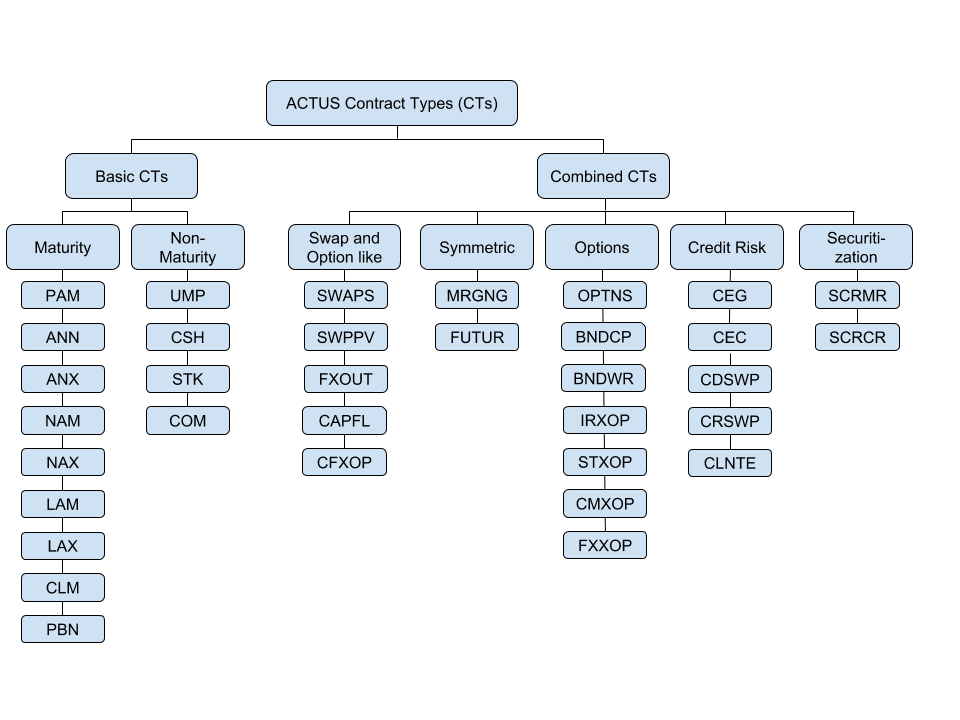
\includegraphics[width=0.45\textwidth]{./media/taxonomy.png}
	\caption{An overview of the ACTUS Contract Types Taxonomy.}
	\label{fig:taxonomy}
\end{figure}


Table \ref{tbl:taxonomy} provides further details on the ACTUS Taxonomy including the real-world financial contracts covered through the various ACTUS Contract Types.


% ---------------------- table: taxonomy ----------------------

% ---------------------- 1-column ----------------------
\end{multicols}

\begin{longtable}{| p{0.07\textwidth}p{0.07\textwidth}p{0.1\textwidth}p{0.45\textwidth}p{0.2\textwidth} |}
	\hline
	\textbf{Family} & \textbf{Class} & \textbf{Type} & \textbf{Description} & \textbf{Covered contracts} \\
	\hline
	\endfirsthead
	\multicolumn{4}{c}{\textit{Continued from previous page}} \\
	\hline
	\textbf{Family} & \textbf{Class} & \textbf{Type} & \textbf{Description} & \textbf{Covered contracts} \\
	\hline
	\endhead
	\hline \multicolumn{4}{r}{\textit{Continued on next page}} \\
	\endfoot
	\endlastfoot
	Basic CT & Maturity & PAM: Principal at Maturity & Principal payment fully at Initial Exchange Date (IED) and repaid at Maturity Date (MD). Fixed and variable rates. & All kind of bonds, term deposits, bullet loans and mortgages etc. \\
	\hline
	 & & ANN: Annuity & Principal payment fully at IED and interest plus principal repaid periodically in constant amounts till MD. If variable rate, total amount for interest and principal is recalculated to be fully matured at MD. & Classical level payment mortgages, leasing contracts etc. \\
	\hline
	 & & NAM: Negative Amortizer & Similar as ANN. However when resetting rate, total amount (interest plus principal) stay constant. MD shifts. Only variable rates. & Special class of ARM´s (adjustable rate mortgages), Certain loans. \\
	\hline
	 & & LAM: Linear Amortizer & Principal payment fully at IED. Principal repaid periodically in constant amounts till MD. Interest gets reduced accordingly. If variable rate, only interest payment is recalculated. Fixed and variable rates. & Many amortizing loans \\
	\hline
	 & & ANX: Exotic Annuity & Exotic version of ANN However step ups with respect to (i) Principal, (ii) Interest rates are possible. Highly flexible to match totally irregular principal payments. Principal can also be paid out in steps. & A special version of this kind are teaser rate loans and mortgages with annuity features \\
	\hline
	 & & LAX: Exotic Linear Amortizer & Exotic version of LAM. However step ups with respect to (i) Principal, (ii) Interest rates are possible. Highly flexible to match totally irregular principal payments. Principal can also be paid out in steps. & A special version of this kind are teaser rate loans and mortgages \\
	\hline
	 & & NAX: Exotic Negative Amortizer & Exotic version of NAM However step ups with respect to (i) Principal, (ii) Interest rates are possible. Highly flexible to match totally irregular principal payments. Principal can also be paid out in steps. & A special version of this kind are teaser rate loans and mortgages with variable MD \\
	\hline
	 & & CLM: Call Money & Loans that are rolled over as long as they are not called. Once called it has to be paid back after the stipulated notice period. & Interbank loans with call features \\
	\hline
	 & & PBN: Perpetual Bonds &  Bonds without any maturity date. Interest is paid into eternity if is not terminated. & Consoles, war loans \\
	\hline
	 & Non-Maturity & UMP: Undefined Maturity Profile & Principal paid in and out at any point in time without prefixed schedule. Interest calculated on outstanding and capitalized periodically. Needs link to a behavioral function describing expected flows. & Saving products of all kind, current accounts. In some countries even variable rate mortgages can be represented with this CT \\
	\hline
	 & & CSH: Cash & Cash or cash equivalent position & Cash, deposits at central bank \\
	\hline
	 & & STK: Stock & Any instrument which is bought at a certain amount (market price normally) and then follows an index. & All straight stocks \\
	\hline
	 & & COM: Commodity & This is not a financial contract in its proper sense. However it tracks movements of commodities such as oil, gas or even houses. Such commodities can serve as underlyings of commodity futures, guarantees or simply asset positions. & Oil, gas, electricity, houses etc. \\
	\hline
	Combined & Swap and Option like & SWAPS: Swap & Exchange of two basic CT´s (PAM, ANN etc.). Normally one is fixed, the other variable. However all variants possible including different currencies for cross currency swaps, basic swaps or even different principal exchange programs. & All kind of swaps. The variety is defined by the underlying CT´s which currently are PAM and ANN in all tis flavors. With each new basic CT the variety rises \\
	\hline
	 & & SWPPV: Plain Vanilla Swap & Plain vanilla swaps where the underlying is always a PAM and one leg is fixed, the other variable. Plain vanilla cross currency swaps also covered. & More than 90\%  of all interest rate swaps follow this simple pattern. \\
	\hline
	 & & FXOUT: Foreign Ex-change Outright & Two parties agree to exchange two fixed cash flows in different currencies at a certain point in time in future. & Any FX-outright transaction. This is also the underlying of FX-options and FX futures \\
	\hline
	 & & CAPFL: Cap Floors & Interest rate option expressed in a maximum or minimum interest rate & Caps and Floor options \\
	\hline
	 & & CFXOP: Exotic Cap Floor & Exotic variants of caps and floors & \\
	\hline
	 & Securiti-zation & SCRMR: Securitized Instruments Market Risk & Instruments bundled and traded in tranches without any specific credit risk feature & MBS, ABS, Principal only, Interest only instruments \\
	\hline
	 & & SCRCR: Securitized instrument Credit Risk Feature & Instruments bundled and traded in tranches that include specific credit risk feature & CDOs \\
	\hline
	 & Symmetric & MRGNG & A generic margining contract governing the agreement of margining usually present at central clearing houses & \\
	\hline
	 & & FUTUR: Future & Keeps track of value changes for any basic CT as underlying (PAM, ANN etc. but also FXOUT, STK, COM). Handles margining calls. & Standard interest rate, FX, stock and commodity futures. \\
	\hline
	 & Options & OPTNS: Option & Calculates straight option pay-off for any basic CT as underlying (PAM, ANN etc.) but also SWAPS, FXOUT, STK and COM. Single, periodic and continuous strike is supported. & European, American and Bermudan options with Interest rate, FX and stock futures as underlying instruments \\
	\hline
	 & & BNDCP: Callable or puttable maturity contract & Bonds with a call or put option. If option is exercised, underlying bond ceases to exist. & Callable and puttable bonds or loans \\
	\hline
	 & & BNDWR: Bond with warrant & Bonds with a warrant. If option is exercised, underlying bond continues to exist. & Warrants \\
	\hline
	 & & IRXOP: Exotic Interest Rate Option & Exotic interest rate options & \\
	\hline
	 & & STXOP: Stock Option & Exotic stock options &  \\
	\hline
	 & & CMXOP: Exotic Commodity Option & Exotic commodity options & \\
	\hline
	 & & FXXOP: Exotic FX Option & Exotic FX options & \\
	\hline
	 & Credit Risk & CEG: Guarantees & Guarantee is a credit enhancement contract. It creates a relationship between a guarantor, an obligee and a debtor, moving the exposure from the debtor to the guarantor. & Personal guarantee. Government guarantee. Underlyings of CDOs. \\
	\hline
	 & & CEC: Collateral & Collateral is a credit enhancement contract. It creates a relationship between a collateral an obligee and a debtor, covering the exposure from the debtor with the collateral. & Mortgages include a collateral contract. Any coverage with financial or physical collateral \\
	\hline
	 & & CDSWP: Credit Default Swap & All sorts of credit default swaps &  \\
	\hline
	 & & CRSWP: Total Return Swap & All sorts of total return swaps & \\
	\hline
	 & & CLNTE: Credit Linked Note & All sorts of credit linked notes & \\
	\hline
	\caption{Financial contract taxonomy}
	\label{tbl:taxonomy}
\end{longtable}


% ---------------------- 2-columns ----------------------
\setlength{\columnsep}{20pt}
\begin{multicols}{2}


%%%%%%%%%%%%%%%%%%%% section: notations %%%%%%%%%%%%%%%%%%%%

\section{Notations}\label{sec:notations}

\subsection{Contract Attributes}\label{sec:attributes}

Contract Attributes (attributes) represent the legal contractual terms that define the exchange of cash-flows of a financial contract. Attributes are introduced by the ACTUS data standard and described in the ACTUS Data Dictionary (DD). Different data types exist and are defined in the DD. In particular, scalar-type and vector-type attributes are defined. Throughout this document the attribute short name is used according to the DD. Further, vector-type attributes may be indexed with a subscript indicating that a specific vector-element is referenced.

\begin{example}[Contract Attribute]
The ACTUS attribute \textit{Initial Exchange Date} is represented in short form \attr{IED}.
\end{example}


\begin{example}[Element of Vector-Type Attribute]
The ACTUS attribute \textit{Array Cycle Anchor Date of Principal Redemption} is a vector-type attribute and represented as \attr{ARPRANX}. The $i$-th element of the vector is referenced by $\attr{ARPRANX}_i$.
\end{example}


\subsection{$\undef$-Operator}\label{sec:undef}

The $\undef$-operator is used to indicate that a certain property is undefined or, in other words, that no value has been assigned to the respective property. In particular, for optional contract attributes it means that the attribute is not defined and for schedule times (see section \ref{sec:schedule}) it means that the respective schedule is empty, i.e. no schedule time defined.

\begin{example}[Undefined Attribute]
$\attr{IPANX}=\undef$ indicates that attribute \attr{IPANX} is undefined.
\end{example}

\begin{example}[Empty Schedule]
$\vec{t}^{IP}=\undef$ means the same as $\vec{t}^{IP}=\{\}$, with $\{\}$ the empty set, and states that the IP schedule $\vec{t}^{IP}$ does not contain a schedule time.
\end{example}


\subsection{$t_0$-Time}\label{sec:t0time}

$t_0$ marks the time as per which the state of a contract is represented in form of the respective set of attributes. Status Date \attr{SD} itself is an attribute of the contract. In general, from the contractual logic we are able to derive any contractual events and contract states for any time $t>t_0$.


\subsection{State Variables}\label{sec:statevarsnotat}

State Variables describe the inner state of a financial contract at a certain point in time $t$ during its lifetime such as (outstanding) Nominal Value, applicable Interest Rate, or the contract performance through Contract Status. State Variables are written in the short form as defined in table \ref{tbl:statevars} with first letter capitalized, printed in bold, and indexed with time.

\begin{example}[State Variables]
$\svar{Nvl}{t}$ refers to the State Variable \textit{Nominal Value} observed at per time $t$.
\end{example}


\subsection{Contract Events}\label{sec:events}

A contract event $e_t^k$ refers to any contractually scheduled or un-scheduled event at a certain time $t$ and of a certain type $k$. Contract events mark specific points in time during the lifetime of a financial contract at which a cash flow is being exchanged (see section \ref{sec:pof}) or the State Variables of the contract are being updated (see section \ref{sec:stf}). Contract Events types $k$ are written in the short form as defined in table \ref{tbl:events}.\\

As an event always has an associated event time $t$ and payoff $c\in\Real$ we define two operators allowing to retrieve these quantities for any single event $e_t^k$ or set of events $\{e_t^k,e_s^j, ...\}$ as follows;

{$\begin{aligned}
	\tev{x} &= \begin{cases} t & \text{if}\quad x=e_t^k \\
				\{t,s,...\} & \text{else if}\quad x=\{e_t^k,e_s^j,...\} \end{cases} \\
	\fev{x} &= \begin{cases} c & \text{if}\quad x=e_t^k \\
				\{c_1, c_2, ...\} & \text{else if}\quad x=\{e_t^k,e_s^j,...\} \end{cases}
\end{aligned}$}

with $c_1=\fev{e_t^k}, c_2=\fev{e_s^j}, ...$.

\begin{example}[Contract Events]
The \textit{Initial Exchange Date} event with event time $s$ is written as $e_s^{IED}$ with $\tev{e_s^{IED}}=s$ and $\fev{e_s^{IED}}=c$ where for any contract type \attr{CT} $c=\pof{IED}{\attr{CT}}$.
\end{example}


\subsection{State Transition Functions}\label{sec:stf}

State Transition Functions (STF) define how the State Variables are being updated when a certain Contract Event $e_t^{k}$ applies from a pre-event (i.e. pre-time $t$) state indexed $t^-$ to a post-event (i.e. post-time $t$) state indexed $t^+$. These functions are specific to a certain Contract Event and Contract Type. STFs are written according to the following pattern \stf{[event type]}{[contract type]} where [event type] and [contract type] refer to the respective event type and contract type to which the STF belongs.

\begin{example}[State Transition Functions]
The STF for an IP event and PAM contract is written as \stf{IP}{PAM} and maps e.g. state variable \textit{Nominal Accrued} from a pre-event state $\svar{Nac}{t^-}$ to post-event state $\svar{Nac}{t^+}$.
\end{example}


\subsection{Payoff Functions}\label{sec:pof}

Payoff Functions (POF) define how the cash flow $c\in\Real$ for a certain Contract Event $e_t^k$ is being derived from current State Variables and Contract Attributes. If necessary, the resulting cash flow can be indexed with the event time $c_t$. These functions are specific to a certain Contract Event and Contract Type. POFs are written according to the following pattern \pof{[event type]}{[contract type]} where [event type] and [contract type] refer to the respective event type and contract type to which the STF belongs.

\begin{example}[Payoff Functions]
The POF for an IP event $e_t^{IP}$ and PAM contract is written as \pof{IP}{PAM} with $\fev{e_t^{IP}}=\pof{IP}{PAM}$.
\end{example}


\subsection{Date/Time}\label{sec:time}

ACTUS builds on the ISO 8601 date/time format. Hence, dates are generally expressed in the following format: [YYYY]-[MM]-[DD]T[hh]:[mm]:[ss].

Time zone information is currently not supported.

A special case is \textit{midnight}. ISO 8601 recognizes both times 00:00:00 and 24:00:00 each referring to midnight. Yet, while 24:00:00 refers to the end of one day, 00:00:00 refers to the beginning of the following day. In ACTUS the interpretation is the same why the time period (measured in any time unit) between the two points in time will always be zero.

For brevity, we use the term \textit{time} for a specific date-time variable and in particular abbreviation Tev for the date of a Contract Event.


\subsection{Event Sequence}\label{sec:eventseq}

Contract Events of different types may occur at the same time, i.e. exactly the same point in time. In this case, the sequence of evaluating their State Transition and Payoff Functions is decisive for the resulting cash flows and state updates. The Event Sequence given for all events in table \ref{tbl:events} defines the order in which these functions are evaluated for the respective event types.


\subsection{Contract Lifetime}\label{sec:lifetime}

The lifetime of an ACTUS contract is the time period of its existence from the perspective of the analyzing user. For every point in time during its lifetime, an ACTUS contract can be analyzed in terms of current State Variables and future cash flows.\\

The lifetime of a contract starts with its \attr{SD} and ends with $\min(MD, AMD, PR^*, STD, TD,\tmax)$.\\

Note that $PR^*$ refers to the PR event of a maturity contract after which \textbf{Nvl}=0.0 (i.e. at which the remaining outstanding principal is redeemed). Further, \attr{MD}, \attr{AMD}, and PR(\textbf{Nvl}=0.0) in the definition above do only apply for maturity contracts but have to be considered infinity in all other cases. Similarly, \attr{STD} only applies for certain contracts and is considered infinity for all others. Finally, $\tmax$ is a parameter that may be used to restrict the considered lifetime in an analysis. In particular, this parameter is used for contracts that do not have a \textit{natural} end to their lifetime such as STK.


%%%%%%%%%%%%%%%%%%%% section: utility functions %%%%%%%%%%%%%%%%%%%%

\section{Utility Functions}\label{sec:utils}


\subsection{Schedule}\label{sec:schedule}

A schedule is a function $S$ mapping times $s,T$ with $s<T$ and cycle $c$ onto a sequence $\vec{t}$ of cyclic times

\[
	\sdl{s}{c}{T}=\vec{t}=\begin{cases} \{\} & \text{if}\quad s=\undef\land T=\undef\\
					s & \text{else if}\quad T=\undef\\
					(s,T) & \text{else if}\quad c=\undef\\
					(s=t_1,...,t_n=T) & \text{else} \end{cases}
\]

with $t_i<t_{i+1}, i=1,2,...$. While the schedule function can be used to create arbitrary sequences of times, it is usually used to generate sequences of cyclic events $\vec{t}^k$ of a certain type $k$, e.g. $k=IP$ for interest payment events (cf. table \ref{tbl:events}) and the following build inputs to the function

\begin{itemize}
	\item[$s$] $=k\attr{ANX}$ with $k\attr{ANX}$ attribute cycle anchor date of event type $k$

	\item[$c$] $=k\attr{CL}$ with $k\attr{CL}$ event type $k$'s schedule cycle

	\item[$T$] $=\attr{MD}$ with \attr{MD} the contract's maturity
\end{itemize}

Thereby, cycles $k\attr{CL}$ have format $NPS$ where

\begin{itemize}
	\item[$N$] is an integer
	\item[$P$] is a time period unit (D=Day, W=Week, M=Month, Q=Quarter, H=Half Year, Y=Year)
	\item[$S$] is a \textit{stub} information ($+$=long last stub, $-$=short last stub)
\end{itemize}

Further, the last stub is defined as follows

\begin{itemize}
	\item[if] $t_{n-1}+c=T \lor S=$'-' then no stub correction applies

	\item[else] $t_n$ is removed from the schedule
\end{itemize}

The sequence of schedule times $\vec{t}^k$ may also be influenced by the \attr{EOF} and \attr{BDC} conventions and the full function syntax becomes $\sdl{s}{c}{T, \attr{EOMC}, \attr{BDC}}$. Due to such effects the sequence of schedule times can be non-equidistant or, in other words, $t_i^k-t_{i-1}^k\neq t_j^k-t_{j-1}^k, i\neq j$.\\

Note that for brevity we will omit the \attr{EOMC} and \attr{BDC} function arguments throughout this document.


\subsection{Array Schedule}\label{sec:arrayschedule}

Array Schedules are defined by vector-valued inputs $\vec{s}=(s_0,s_1,...,s_m)$ and $\vec{c}=(c_0,c_1,...,c_m)$ to the regular schedule function

\begin{multline*}
	\sdl{\vec{s}}{\vec{c}}{T} = (\sdl{s_0}{c_0}{s_1-c_0},\\
					\sdl{s_1}{c_1}{s_2-c_1},...,\sdl{s_m}{c_m}{T})
\end{multline*}


Hence, array schedules are a generalization for regular schedules which coincide for $m=1$. In accordance with regular schedules \attr{EOMC} and \attr{BDC} conventions also apply here.


\subsection{End Of Month Shift Convention}\label{sec:eomc}

For schedules $\vec{t}^k$ starting at time $s$ which marks the end of a month with 30 or less days, e.g. April 30, and with a cycle $c$ being a multiple of 1M- attribute \attr{EOM} defines whether the schedule times are to fall on the 30th of all months (same day) or the 31st (end of month).\\

More specifically, \attr{EOM} has an effect on a schedule $\vec{t}^k$ only if:

\begin{itemize}
	\item[$s$] is the last day of a month with less than 31 days (Feb, April etc.)

	\item[$c$] $=NPS$ with $P\in(M, Q, H or Y)$
\end{itemize}

As per the DD \attr{EOM} can take one of the following values:
\begin{itemize}
	\item[EOM] (EndOfMonth): times $t_i,i=1,2,...,n-1$ are moved to the end of the respective months

	\item[SD] (SameDay): times $t_i,i=1,2,...,n-1$ remain unchanged except in February, where it will go to the last day if the day of month of time $s$ is higher than the number of days of February
\end{itemize}


\subsection{Business Day Shift Convention}\label{sec:bdc}

In general, contract events are scheduled for business days only. Therefore, the \attr{BDC} convention defines how scheduled times $t_i,i=1,2,...,n-1$ are shifted in case they fall on a non-business day:

\begin{itemize}
	\item[NULL:] No shift

	\item[SCF:] Shift/Calculate following: The event is shifted to the following non working day. Calculation of the event happens after the shift

	\item[SCMF:] Shift/Calculate modified following: The event is shifted to the following non working day. However, if the following day happens to fall into the next month, then take preceeding non-working day. Calculation of the event happens after the shift

	\item[CSF:] Calculate/Shift following: Same like SCF however calculation of the event happens before the shift

	\item[CSMF:] Calculate/Shift modified following: Same like SCMF however calculation of the event happens before the shift

	\item[SCP:] Shift/Calculate preceding: The event is shifted to the last preceding non working day. Calculation of the event happens after the shift

	\item[SCMP:] Shift/Calculate modified preceding: The event is shifted to the last preceding non working day. However, if the preceding day happens to fall into the previous month, then take next non-working day. Calculation of the event happens after the shift

	\item[CSP:] Calculate/Shift preceding: Same like SCP however calculation of the event happens before the shift

	\item[CSMP:] Calculate/Shift modified preceding: Same like SCMP however calculation of the event happens before the shift
\end{itemize}


\subsection{Business Day Calendar}\label{sec:bdcal}

Whether a specific day is a business day (cf. previous section) is defined by attribute \attr{CLDR}. Such conventions generally depend on regional official holiday calendars. The Business Day Function interface allows determining for some \attr{CLDR} whether any time $t$ is a business day or not

\[
	B: t \mapsto \{true, false\}
\]

where $true$ indicates that $t$ is a business day and $false$ that it is a holiday.


\begin{example}
Two standard \attr{CLDR} implementations are the following
\begin{itemize}
	\item NoHoliday (default): every calendar day is a business day

	\item MondayToFriday: all weekdays Monday, Tuesday, Wednesday, Thursday, and Friday are business days
\end{itemize}
\end{example}


\subsection{Year Fraction Convention}\label{sec:yearfrac}

Interest income and other calculations are based on \textit{per annum} interest rates. Therefore, the year-fraction function interface $Y$ is used to calculate the \textit{fraction of a year} between any two times $s$ and $t$ with $t>s$ for which e.g. an (per annum) interest rate applies according to some day count convention \attr{DCC}

\[
	\yfrfunc: s,t,\attr{DCC} \mapsto \Real
\]

Note, the year fraction function interface only defines the structure of year fraction functions but not an actual implementation thereof, or the respective \attr{DCC}, respectively. Therefore, any \attr{DCC} can be implemented according to the interface above supporting user-defined year fraction functions.\\

For brevity we will omit the \attr{DCC} function argument wherever this does not lead to confusion.


\subsection{Contract Role Sign Convention}\label{sec:cntrl}

The two counterparties to a financial contract are defined through attributes \attr{LEIRC} and \attr{LEICP}. The first is the party initially \textit{creating} the contract and the second is the counterparty, respectively. Thereby, both \attr{LEIRC}/\attr{LEICP} can take any \textit{role} in the contract or, more specifically, they can be the lender or borrower in a loan (PAM), fixed receiver or payer in an interest rate swap (SWAPS), etc.\\

The \textit{role} of the \attr{LEIRC} is defined through attribute \attr{CNTRL}. The \textit{role} of \attr{LEICP} is derived as the \textit{opposite} side to the contract. Apart from \attr{CNTRL} the attributes are \textit{neutral} to the \textit{role} of \attr{LEIRC} (or \attr{LEICP}).\\

On the other hand, contractual cash flows generated by the POFs and certain state variables are \textit{role-sensitive}. That is, from the perspective of the \attr{LEIRC} these quantities represent either claims or obligations. Contract Role Sign function $R$ maps the \attr{CNTRL} attribute into $+1$ indicating a claim or $-1$ indicating an obligation

\[
	R : \attr{CNTRL} \rightarrow \{-1, +1 \}
\]

When multiplying with a cash flow $x$ the Contract Role Sign function thereby defines the direction of that flow:

\begin{itemize}
	\item[$x>0$:] $x$ flows from \attr{LEICP} to \attr{LEIRC}

	\item[$x<0$:] $x$ flows from \attr{LEIRC} to \attr{LEICP}
\end{itemize}

Table \ref{tbl:cntrl} defines the domain of the Contract Role Sign function, i.e. the range of attribute \attr{CNTRL}, with meaning and Contract Role Sign to which the function maps.


% ---------------------- table: contract roles ----------------------
\begin{table}[H]
	\centering
	\begin{tabular}{| p{0.5in}p{1.5in}p{0.2in} |}
	\hline
	\textbf{Value} & \textbf{Meaning} & $\textbf{R}$ \\
	\hline
	RPA & Real position asset & +1 \\
	\hline
	RPL & Real position liability & -1 \\
	\hline
	CLO & Role of a collateral & +1 \\
	\hline
	CNO & Role of a close-out-netting & +1 \\
	\hline
	COL & Role of an underlying to a collateral & +1 \\
	\hline
	LG & Long position & +1 \\
	\hline
	ST & Short position & -1 \\
	\hline
	BUY & Protection buyer & +1 \\
	\hline
	SEL & Protection seller & -1 \\
	\hline
	RFL & Receive first leg & +1 \\
	\hline
	PFL & Pay first leg & -1 \\
	\hline
	RF & Receive fix leg & +1 \\
	\hline
	PF & Pay fix leg & -1 \\
	\hline
	\end{tabular}
	\caption{Contract Role definitions.}
	\label{tbl:cntrl}
\end{table}


\subsection{Contract Default Convention}\label{sec:default}

Performance of a contract indicates whether as per a certain time all parties involved adhere to their obligations arising from the contract. Attribute \attr{CTS} captures a contract's performance as per $t_0$. For any time $t>t_0$ and depending on the behavior of the parties involved the contract can migrate into different contract (performance) statuses from \textit{'performing'} to \textit{'default'}. State variable $\svar{Prf}{t}$ (cf. table \ref{tbl:statevars}) captures these dynamics and the performance as per any time $t>t_0$.\\

The Contract Default Convention is a function $D$ that maps the $\svar{Prf}{t}$ state variable into $+1$ indicating that the contract is performing or $0$ which reflext default and, from an analytical perspective, means that future cash flows \textit{cancel out}:

\[
\dfl{t} = \begin{cases} 1 & \text{if} \quad \svar{Prf}{t}\neq \text{'D'} \\
				0 & \text{else} \end{cases}
\]


\subsection{Annuity Amount Function}\label{sec:annamount}

In an \textit{Annuity} contract (ANN) the annuity amount is paid regularly from the \textit{borrower} to the \textit{lender}. Thereby, the annuity amount is comprised of a principal repayment portion and an interest portion and and dimensioned such that the total nominal amount $n$ at time $t$ is fully repaid at maturity $T$ of the annuity. The Annuity Amount function $\ann$ computes the annuity amount as follows

\[
	\ann{s}{T}{n}{a}{r}=(n+a)\frac{\prod_{i=1}^{m-1}1+r\yfr{t_i,t_{i+1}}}{1+\sum_{i=1}^{m-1}\prod_{j=i}^{m-1}1+r\yfr{t_j}{t_{j+1}}}
\]

with $a$ the accrued interest as per time $s$, $r$ the actual interest rate, $t_i, i=1,2,...,m$ the schedule times $\inf t, t\in\vec{t}^{PR}\land t>s$, $m$ the number of times $t_i$, and $\vec{t}^{PR}$ the PR-event schedule times of the Annuity contract as described in section \ref{sec:ann}.


\subsection{Canonical Contract Payoff Function}

The canonical payoff of a contract $x$ is defined as the sum of all future event payoffs evaluated under current risk factor conditions, or

\[
  \payoff{x}{t} = \sum_{c\in C} c
\]

with $C=\fev{\cldev{x}{t}{\obs{rf}{\attr{i}}{s}=\obs{rf}{\attr{i}}{t}\forall i \wedge s>t}}$.

%%%%%%%%%%%%%%%%%%%% section: state variables %%%%%%%%%%%%%%%%%%%%

\section{Contract State Variables}\label{sec:statevars}

Driven by Contract Events (see section \ref{sec:events}) certain contractual dimensions, state variables, of financial contracts may change during the lifetime of a financial contract. Thereby, the set of State Variables varies for different CTs. Table \ref{tbl:statevars} represents the set of all covered State Variables throughout the universe of CTs.\\

By definition, State Variables are updated through Contract Events only. The value of State Variables always shows the state of the contract \textbf{after} the respective Contract Event.


% ---------------------- table: state variables ----------------------
\begin{table}[H]
	\centering
	\begin{tabular}{| p{0.8in}p{0.3in}p{1.8in} |}
	\hline
	\textbf{Name} & \textbf{Abbrv.} & \textbf{Explanation} \\
	\hline
	Performance & $\svar{Prf}{t}$ & Contract performance \\
	\hline
	Last Event Date & $\svar{Led}{t}$ & The date of the most recent Contract Event \\
	\hline
	Nominal Value & $\svar{Nvl}{t}$ & The outstanding nominal value \\
	\hline
	Secondary Nominal Value & $\svar{Nv2}{t}$ & The outstanding nominal value of the second leg \\
	\hline
	Nominal Rate & $\svar{Nrt}{t}$ & The applicable nominal rate \\
	\hline
	Nominal Accrued & $\svar{Nac}{t}$ & The current value of nominal accrued interest at the Nominal Rate \\
	\hline
	Interest Calculation Base & $\svar{Icb}{t}$ & The basis at which interest is being accrued if different from $\svar{Nvl}{t}$ \\
	\hline
	Notional Scaling Multiplier & $\svar{Nsc}{t}$ & The multiplier being applied to Notional/Principal related
	cash-flows \\
	\hline
	Interest Scaling Multiplier & $\svar{Isc}{t}$ & The multiplier being applied to Interest related cash-flows \\
	\hline
	Next Principal Redemption Payment & $\svar{Npr}{t}$ & The value at which $\svar{Nvl}{t}$ is being repaid. This may be including or excluding of interest depending on the instrument\\
	\hline
	Payoff at Settlement & $\svar{Pos}{t}$ & The payoff of the contract if fixed at time $t$. If evaluated during the lifetime of the contract this quantity gives a hypothetical payoff (e.g. for an OPTNS contract it defines whether the option is in-the-money or not).\\
	\hline
	\end{tabular}
	\caption{State variables}
	\label{tbl:statevars}
\end{table}



%%%%%%%%%%%%%%%%%%%% section: events %%%%%%%%%%%%%%%%%%%%

\section{Contract Event Types}\label{sec:eventtypes}

An overview and description of various event types can be found in table \ref{tbl:events}.

\end{multicols}

% ---------------------- table: events ----------------------
\begin{longtable}{| p{0.07\textwidth}p{0.3\textwidth}p{0.51\textwidth}p{0.05\textwidth} |}
	\hline
	\textbf{Type} & \textbf{Name} & \textbf{Explanation} & \textbf{Seq.} \\
	\hline
	\endfirsthead
	\multicolumn{4}{c}{\textit{Continued from previous page}} \\
	\hline
	\textbf{Type} & \textbf{Name} & \textbf{Explanation} & \textbf{Seq.} \\
	\hline
	\endhead
	\hline \multicolumn{4}{r}{\textit{Continued on next page}} \\
	\endfoot
	\endlastfoot
	IED & Initial Exchange Date & Scheduled date of first principal event, start of accrual calculation & 1 \\
	\hline
	IPCI & Interest Capitalization & Scheduled interest payment which is capitalized instead of paid out & 2 \\
	\hline
	IP & Interest Payment & Scheduled interest payment & 3 \\
	\hline
	FP & Fee Payment & Scheduled fee payment & 4 \\
	\hline
	PR & Principal Redemption & Scheduled principal redemption payment & 5 \\
	\hline
	PI & Principal Increase & Scheduled principal increase payments & 6 \\
	\hline
	PRF & Principal Payment Amount Fixing & Scheduled re-fixing of principal payment (PR or PI) amount & 7 \\
	\hline
	PY & Penalty Payment & Payment of a penalty (e.g. due to early repayment of principal outstanding) & 8 \\
	\hline
	PP & Principal Prepayment & Unscheduled (early) repayment of principal outstanding & 9 \\
	\hline
	CD & Credit Default & Credit event of counterparty to a contract & 10 \\
	\hline
	RRF & Rate Reset Fixed & Scheduled rate reset event where new rate is already fixed & 11 \\
	\hline
	RR & Rate Reset Variable & Scheduled rate reset event where new rate is fixed at event time & 12 \\
	\hline
	DV & Dividend Payment & Scheduled (e.g. announced) dividend payment & 13 \\
	\hline
	PRD & Purchase Date & Purchase date of a contract bought in the secondary market & 14 \\
	\hline
  IMP & Initial Margin Payment & Initial margin call event  & 15 \\
	\hline
	MP & Margin Payment & Scheduled margin call event & 16 \\
	\hline
	TD & Termination Date & Sell date of a contract sold in the secondary market & 17 \\
	\hline
	SC & Scaling Index Revision & Scheduled re-fixing of a scaling index & 18 \\
	\hline
	IPCB & Interest Payment Calculation Base & Scheduled update to the calculation base for IP accruing & 19 \\
	\hline
	XD & Execution Date & Scheduled or unscheduled execution of e.g. an OPTNS or FUTUR contract & 20 \\
	\hline
	STD & Settlement Date & Date when payment for derivatives is settled & 21 \\
	\hline
	MD & Maturity Date & Scheduled maturity or expiry of a contract & 22 \\
	\hline
	AD & Analysis Event & Retrieves current contract states without alter these & 23 \\
	\hline
	%\end{tabular}
	\caption{Contract Events Definitions.}
	\label{tbl:events}
\end{longtable}


% ---------------------- 2-columns ----------------------
\setlength{\columnsep}{20pt}
\begin{multicols}{2}


%%%%%%%%%%%%%%%%%%%% section: contract composition %%%%%%%%%%%%%%%%%%%%

\section{Contract Composition}\label{sec:composition}

The payoff of \textit{Combined Contracts}, see the taxonomy in \ref{fig:taxonomy}, is derived from certain quantities of child contracts (also called \textit{underlying instruments} or simply \textit{underlyers}). In general, such child contracts can be any ACTUS contract - Basic or Combined - as well as any number of contracts - a single contract or a set of contracts. Indeed, in reality this is what Option, Swap, Swaption, but also any kind of Asset/Mortgage/etc. backed securities represent; \textit{a hierarchical composition of different contracts linked by means of functional reationships}. This compositional approach provides maximum flexibility and, hence, allows capturing any real world use case. We here refer to a \textit{referenced} (i.e. of lower hierarchical level) contract as a \textit{child contract} and to a referencing (i.e. of higher hierarchical level) contract as a \textit{parent contract}.\\

The ACTUS DD defines attribute $\attr{CTST}$ which captures the child contract(s) as part of the parent contract's set of attributes. Thereby, attribute $\attr{CTST}$ is of type \textit{ContractStructure} which is a simple structure of the form (in JSON notation)

\begin{verbatim}
{
"ContractReference":[ r1, r2, ... ]
}
\end{verbatim}

where the \verb'r1', \verb'r2', ... refer to objects of type \textit{ContractReference} (in JSON notation)

\begin{verbatim}
{
"Object": ,
"Type": ,
"Role":
}
\end{verbatim}

with fields

\begin{itemize}
	\item[] \verb'Object': an object representing the reference
	\item[] \verb'Type': one of the values listed in table \ref{tbl:struct-types}
	\item[] \verb'Role': one of the values listed in table \ref{tbl:struct-roles}
\end{itemize}


% ---------------------- table: contract structure types ----------------------
\begin{table}[H]
	\centering
	\begin{tabular}{| p{1.2in}p{1.7in} |}
	\hline
	\textbf{Type} & \textbf{Explanation} \\
	\hline
	Contract & The reference represents an actual contract \\
	\hline
	ContractIdentifier & The reference represents an identifier of an actual contract \\
	\hline
	MarketObjectIdentifier & The reference represents the identifier of a market object (e.g. price feed) \\
	\hline
	LegalEntityIdentifier & The reference represents the identifier of a legal entity \\
	\hline
	ContractStructure & The reference represents a ContractStructure \\
	\hline
	\end{tabular}
	\caption{ContractReference types}
	\label{tbl:struct-types}
\end{table}


% ---------------------- table: contract structure roles ----------------------
\begin{table}[H]
	\centering
	\begin{tabular}{| p{1.0in}p{1.4in}p{0.5in} |}
	\hline
	\textbf{Role} & \textbf{Explanation} & \textbf{Contract} \\
	\hline
	Underlying & The reference represents a simple underlyer contract & FUTUR, OPTNS \\
	\hline
	FirstLeg & The reference represents the first leg contract & SWAPS \\
	\hline
	SecondLeg & The reference represents the second leg contract & SWAPS \\
	\hline
	CoveredContract & The reference represents a contract that is covered under the parent contract & CEG, CEC \\
	\hline
	CoveringContract & The reference represents a contract that covers for covering contracts under the parent contract & CEC \\
	\hline
	\end{tabular}
	\caption{ContractReference roles}
	\label{tbl:struct-roles}
\end{table}


We will use the following notation to query reference objects from the $\attr{CTST}$ attribute

\[
	\attr{CTST}_{role}^{type}(i)
\]

where $type$ identifies the references (\verb'r1', \verb'r2', ...) with \verb'type'=$type$, $role$ the reference with \verb'Role'=$role$, and $i$ identifies the $i$'th element of the queried references. For brevity, we will omit the index parameter $i$ which indicates that we address the first (and usually only) reference object queried.

\begin{example}[Underlying MarketObject-reference] The MarketObject reference of a simple Underlying e.g. to an Option contract is referenced as $\attr{CTST}_{Underlying}^{MarketObjectIdentifier}(1)$ or, in short form, as $\attr{CTST}_{Underlying}^{MarketObjectIdentifier}$.
\end{example}

\begin{example}[FirstLeg Contract-reference] The Contract object representing the first leg e.g. to a Swaps contract is referenced as $\attr{CTST}_{FirstLeg}^{Contract}(1)$ or, in short form, as $\attr{CTST}_{FirstLeg}^{Contract}$.
\end{example}


%%%%%%%%%%%%%%%%%%%% section: risk factor observer %%%%%%%%%%%%%%%%%%%%

\section{Risk Factor Observer}\label{sec:rfobserver}

The payoff of financial contracts always depends on the context in which it is evaluated and which is comprised of the following dimensions; counterparties, markets, and behavioral factors. We refer to these as the \textit{risk factors} to which financial contracts are exposed to. This indicates that these factors are source of uncertainty because financial contracts only reference the factors but their dynamics is outside the control of any contractual agreement. Thus, such factors have to be \textit{observed} and their changing states accounted for when evaluating the payoff of financial contracts. Therefore, we consider a standardized interface $\obsfull{o}{i}{t}{S}{M}$ that allows for \textit{observing}; (1) the state of a certain risk factor $i$ at any time $t$ if $o=$'rf'

\[
	\obsfunc{rf}: i,t,S,M \mapsto \Real
\]

and (2) contractual but non-scheduled events if $o=$'ev'

\[
	\obsfunc{ev}: i,t,S,M \mapsto \{e_t^{k},e_s^{l},...\}
\]

The parameters to the Risk Factor Observer interface are as follows:

\begin{itemize}
	\item[$i$]: the identifier of the risk factor \textit{observed}

	\item[$t$]: the time for which the risk factor’s state should be evaluated

	\item [$S$]: the inner states of the contract at time $t$

	\item [$M$]: the contract terms of the contract as per time $t$
\end{itemize}

Note that the observer interface only defines the structure of an actual observer function but not the actual implementation. Thus, the interface allows for user-defined implementations of observer functions allowing e.g. for representing arbitrary assumptions on the evolution of future risk factor states which is key for any type of forward-looking analysis.

\begin{example}['rf'-Observer] The market-driven 3-month USD-Libor reference rate used as the variable rate in a variable rate loan contract is observed at any time $t$ through $\obs{rf}{\attr{MarketObjectCodeRateReset}}{t}$.
\end{example}

\begin{example}['rf'-Observer] Unscheduled (pre-) repayments of outstanding notional in a mortgage contract is observed at any time $t$ through $\obs{ev}{\attr{CID}}{t}$.
\end{example}

For brevity we will omit the $S$ and $M$ function arguments wherever this does not lead to confusion.


%%%%%%%%%%%%%%%%%%%% section: child observer %%%%%%%%%%%%%%%%%%%%

\section{Child Contract Observer}\label{sec:cldobserver}

In order to evaluate the derived payoff of combined contracts, we consider a standardized interface $\cldfunc{o}$ that allows for \textit{observing} on the parent level; (1) all future events, w.r.t. time $t$, if $o=$'ev'

\[
	\cldfunc{ev}: i,t,a \mapsto \{e_v^{k},e_w^{l},...\}
\]

with $v,w>t$ and event types $k,l$ according to the schedule of the child contract, (2) a certain state variable $x$ if $o=$'sv'

\[
	\cldfunc{sv}: i,t,x,a \mapsto \Real,
\]

or (3) a particular contract attribute $x$ of the child contract if $o=$'ca'

\[
	\cldfunc{ca}: i,x \mapsto y
\]

with $y$ a variable of value type of the respective attribute as per DD.\\

The parameters to the Child Contract Observer interface are as follows:

\begin{itemize}
	\item[$i$]: the identifier of the child contract \textit{observed}

	\item[$t$]: for $o\in\{\textit{ev,sv}\}$ the time for which the respective quantity should be evaluated

	\item [$x$]: for $o\in\{\textit{sv,ca}\}$ the quantity to be evaluated

	\item [$a$]: for $o\in\{\textit{ev,sv}\}$ a set of contract attributes to which the evaluated quantity should be conditioned
\end{itemize}


Note that the observer interface only defines the structure of an actual observer function but not the actual implementation. Thus, the interface allows for user-defined implementations of observer functions allowing e.g. for using arbitrary data structures.

\begin{example}['ev'-Observer] The future events, w.r.t. time $t$, of the \textit{first leg} (i.e. child contract with \verb'Role'=$\texttt{FirstLeg}$) of a SWAPS contract with $\attr{CNTRL}=PFL$ (i.e. \textit{pay first leg}) can be evaluated as $\cldev{\attr{CTST}_{FirstLeg}^{Contract}}{t}{\attr{CNTRL}=RPL}$.
\end{example}

\begin{example}['sv'-Observer] The current state, w.r.t. time $t$, of state variable $\svar{Nvl}{}$ of the \textit{first leg} (i.e. child contract with \verb'Role'=$\texttt{FirstLeg}$) of a SWAPS contract with \attr{CNTRL}=RFL (i.e. \textit{receive first leg}) can be evaluated as $\cldsv{\attr{CTST}_{FirstLeg}^{Contract}}{t}{Nvl}{\attr{CNTRL}=RPA}$.
\end{example}

\begin{example}['ca'-Observer] The contract attribute \attr{MOC} of the child contract \textit{Child} (i.e. child contract with \verb'Role'=$\texttt{Underlying}$) of an OPTNS contract can be evaluated as $\cldca{\attr{CTST}_{Underlying}^{Contract}}{\attr{MOC}}$.
\end{example}

For brevity we will omit the $x$ and $a$ function arguments wherever this does not lead to confusion.



%%%%%%%%%%%%%%%%%%%% section: contract types %%%%%%%%%%%%%%%%%%%%

% ---------------------- 1-column ----------------------
\end{multicols}

% ---------------------- newpage ----------------------
\newpage

\section{Contract Types}\label{sec:contracts}



%%%%%%%%%%%%%%%%%%%% subsection: pam %%%%%%%%%%%%%%%%%%%%

\subsection{PAM: Principal At Maturity}\label{sec:pam}


% ---------------------- table: pam schedule ----------------------
\begin{schedule}{PAM}
	AD & $\vec{t}^{AD} = \left(t_0,t_1,...,t_n\right)$ & With $t_i,i=1,2,...$ a custom input \\
	\hline
	IED & $t^{IED} = \attr{IED}$ & \\
	\hline
	PR & $t^{PR} = \svar{Tmd}{t_0}$ & \\
	\hline
	PP & $\vec{t}^{PP} = \begin{cases} \undef & \text{if} \quad \attr{PPEF}=\text{'N'} \\
					(\vec{u},\vec{v}) & \text{else} \end{cases}$
		\par where \par
		{$\begin{aligned} \vec{u} &= \sdl{s}{\attr{OPCL}}{T^{MD}} \\
				\vec{v} &= \obs{rf}{\attr{PPMO}}{t} \end{aligned}$}
		 & with\par $s = \begin{cases} \undef & \text{if} \quad \attr{OPANX}=\undef \land \attr{OPCL}=\undef\\
					   \attr{IED}+\attr{OPCL} & \text{else if} \quad \attr{OPANX} = \undef \\
					   \attr{OPANX} & \text{else} \end{cases}$ \\
	\hline
	PY & $\vec{t}^{PY} = \begin{cases} \undef & \text{if} \quad \attr{PYTP}=\text{'O'} \\
						\vec{t}^{PP} & \text{else} \end{cases}$ & \\
	\hline
	FP & $\vec{t}^{FP} = \begin{cases} \undef & \text{if} \quad \attr{FER}=\undef \lor \attr{FER}=0 \\
					\sdl{s}{\attr{FPCL}}{T^{MD}} & \text{else} \end{cases}$
		& with\par $s = \begin{cases} \undef & \text{if} \quad \attr{FPANX}=\undef \land \attr{FPCL}=\undef\\
					   \attr{IED}+\attr{FPCL} & \text{else if} \quad \attr{FPANX} = \undef \\
					   \attr{FPANX} & \text{else} \end{cases}$ \\
	\hline
	PRD & $t^{PRD}= \attr{PRD}$  &  \\
	\hline
	TD & $t^{TD}= \attr{TD}$  &  \\
	\hline
	IP & $\vec{t}^{IP} = \begin{cases} \undef & \text{if} \quad \attr{IPNR}=\text{'O'} \\
						\sdl{s}{\attr{IPCL}}{T^{MD}} & \text{else} \end{cases}$
		& with\par $s = \begin{cases} \undef & \text{if} \quad \attr{IPANX}=\undef \land \attr{IPCL}=\undef\\
					\attr{IPCED} & \text{else if}\quad \attr{IPCED}\neq\undef \\
					   \attr{IED}+\attr{IPCL} & \text{else if} \quad \attr{IPANX} = \undef \\
					   \attr{IPANX} & \text{else} \end{cases}$ \\
	\hline
	IPCI & $\vec{t}^{IPCI} = \begin{cases} \undef & \text{if} \quad \attr{IPCED}=\undef \\
						\sdl{s}{\attr{IPCL}}{\attr{IPCED}} & \text{else} \end{cases}$
		& with\par $s = \begin{cases} \undef & \text{if} \quad \attr{IPANX}=\undef \land \attr{IPCL}=\undef\\
					   \attr{IED}+\attr{IPCL} & \text{else if} \quad \attr{IPANX} = \undef \\
					   \attr{IPANX} & \text{else} \end{cases}$ \\
	\hline
	RR & $\vec{t}^{RR} = \begin{cases} \undef & \text{if} \quad \attr{RRANX}=\undef \land \attr{RRCL}=\undef \\
					\vec{t} \setminus t^{RRY} & \text{else if} \attr{RRNXT} \neq \undef \\
					\vec{t} & \text{else} \end{cases}$ \par
		where $\vec{t}=\sdl{s}{\attr{RRCL}}{T^{MD}}$
		& with\par {$\begin{aligned} s &= \begin{cases} \attr{IED}+\attr{RRCL} & \text{if} \quad \attr{RRANX} = \undef \\
					   \attr{RRANX} & \text{else} \end{cases} \\
					     t^{RRY} &= \inf t \in \vec{t}\mid t>\attr{SD} \end{aligned}$} \\
	\hline
	RRF & $t^{RRF} = \begin{cases} \undef & \text{if} \quad \attr{RRANX}=\undef \land \attr{RRCL}=\undef \\
					\inf t \in \vec{t}\mid t>\attr{SD} & \text{else} \end{cases}$ \par
		where $\vec{t}=\sdl{s}{\attr{RRCL}}{T^{MD}}$
		& with\par $s = \begin{cases} \attr{IED}+\attr{RRCL} & \text{if} \quad \attr{RRANX} = \undef \\
					   \attr{RRANX} & \text{else} \end{cases}$ \\
  	\hline
	SC & $\vec{t}^{SC} = \begin{cases} \undef & \text{if} \quad \attr{SCEF}=\text{'000'} \\
					\sdl{s}{\attr{SCCL}}{T^{MD}} & \text{else} \end{cases}$
		& with\par $s = \begin{cases} \undef & \text{if} \quad \attr{SCANX}=\undef \land \attr{SCCL}=\undef\\
					   \attr{IED}+\attr{SCCL} & \text{else if} \quad \attr{SCANX} = \undef \\
					   \attr{SCANX} & \text{else} \end{cases}$ \\
	\hline
	CD & $t^{CD} = \obs{ev}{LEICP}{t_0}$ & \\
\end{schedule}


% ---------------------- table: pam states ----------------------
\begin{states}{PAM}
	$\svar{Tmd}{}$ & $\svar{Tmd}{t_0} = \attr{MD}$ & \\
	\hline
  	$\svar{Nvl}{}$ & $\svar{Nvl}{t_0} = \begin{cases} 0.0 & \text{if} \quad \attr{IED} > t_0 \\
							\sgn\times\attr{NT} & \text{else} \end{cases}$ & \\
	\hline
	$\svar{Nrt}{}$ & $\svar{Nrt}{t_0} = \begin{cases} 0.0 & \text{if} \quad \attr{IED} > t_0 \\
							\attr{IPNR} & \text{else} \end{cases}$ & \\
  	\hline
  	$\svar{Nac}{}$ & $\svar{Nac}{t_0} = \begin{cases} 0.0 & \text{if} \quad \attr{IPNR}=\undef \\
							\attr{IPAC} & \text{else if} \quad \attr{IPAC} \neq \undef \\
							\yfr{t^-}{t_0}\times\svar{Nvl}{t_0}\times\svar{Nrt}{t_0} & \text{else} \end{cases}$ &
			with $t^- = \sup t \in \vec{t}^{IP}\mid t<t_0$ \\
	\hline
  	$\svar{Fac}{}$ & $\svar{Fac}{t_0} = \begin{cases} 0.0 & \text{if} \quad \attr{FER}=\undef \\
					\attr{FEAC} & \text{else if} \quad \attr{FEAC} \neq \undef \\
					\yfr{t^-}{t_0}\times\svar{Nvl}{t_0}\times\attr{FER} & \text{else if} \quad \attr{FEB}=\text{'N'} \\
					\frac{\yfr{t^{FP-}}{t_0}}{\yfr{t^{FP-}}{t^{FP+}}}\times\attr{FER} & \text{else} \end{cases}$ &
			with {$\begin{aligned} t^{FP-} &= \sup t \in \vec{t}^{FP}\mid t<t_0 \\
						t^{FP+} &= \inf t \in \vec{t}^{FP}\mid t>t_0 \end{aligned}$} \\
  	\hline
  	$\svar{Nsc}{}$ & $\svar{Nsc}{t_0} = \begin{cases} \attr{SCIXSD} & \text{if} \quad \attr{SCEF}=\text{'[x]N[x]'} \\
					1.0 & \text{else} \end{cases}$ & \\
  	\hline
  	$\svar{Isc}{}$ & $\svar{Isc}{t_0} = \begin{cases} \attr{SCIXSD} & \text{if} \quad \attr{SCEF}=\text{'I[x][x]'} \\
					1.0 & \text{else} \end{cases}$ & \\
	\hline
  	$\svar{Prf}{}$ & $\svar{Prf}{t_0} = \attr{CTS}$ &  \\
	\hline
	$\svar{Led}{}$ & $\svar{Led}{t_0} = t_0$ & \\
\end{states}


% ---------------------- table: pam functions ----------------------
\begin{functions}{PAM}
	AD & 0.0 & {$\begin{aligned}
				\svar{Nac}{t^+} &= \svar{Nac}{t^-} + \yfr{\svar{Led}{t^-1}}{t}\svar{Nrt}{t^-}\svar{Nvl}{t^-}\\
				\svar{Led}{t^+} &= t
			\end{aligned}$} \\
	\hline
	IED & $\dfl{t^-}\sgn(-1)(\attr{NT}+\attr{PDIED})$
		& {$\begin{aligned}
			\svar{Nvl}{t^+} &=\sgn\attr{NT} \\
			\svar{Nrt}{t^+} &= \begin{cases} 0.0 & \text{if} \quad \attr{IPNR}=\undef \\
							\attr{IPNR} & \text{else} \end{cases} \\
			\svar{Nac}{t^+} &= \begin{cases} \attr{IPAC} & \text{if} \quad \attr{IPAC} \neq \undef \\
							y\svar{Nvl}{t^+}\svar{Nrt}{t^+} & \text{if} \quad \attr{IPANX} \neq \undef \land \attr{IPANX}<t \\
							0.0 & \text{else} \end{cases} \\
			\svar{Led}{t^+} &= t \end{aligned}$}\par
		with\par
		$y=\yfr{\attr{IPANX}}{t}$ \\
	\hline
	PR & $\dfl{t^-}\svar{Nsc}{t^-}\svar{Nvl}{t^-}$
		& {$\begin{aligned}
			\svar{Nvl}{t^+} &= 0.0 \\
			\svar{Nrt}{t^+} &= 0.0 \\
			\svar{Led}{t^+} &= t \end{aligned}$} \\
	\hline
	PP & $\dfl{t^-}\obs{rf}{\attr{OPMO}}{t}$
		& {$\begin{aligned}
			\svar{Nac}{t^+} &= \svar{Nac}{t^-} + \yfr{\svar{Led}{t^-}}{t}\svar{Nrt}{t^-}\svar{Nvl}{t^-} \\
			\svar{Fac}{t^+} &= \begin{cases} \svar{Fac}{t^-} + \yfr{\svar{Led}{t^-}}{t}\svar{Nvl}{t^-}\attr{FER} & \text{if} \quad \attr{FEB}=\text{'N'} \\
					\frac{\yfr{t^{FP-}}{t}}{\yfr{t^{FP-}}{t^{FP+}}}\attr{FER} & \text{else} \end{cases} \\
			\svar{Nvl}{t^+} &= \svar{Nvl}{t^-} - \obs{rf}{\attr{OPMO}}{t} \\
			\svar{Led}{t^+} &= t \end{aligned}$} \par
		with\par
		{$\begin{aligned}
			t^{FP-} &= \sup t \in \vec{t}^{FP}\mid t<t_0 \\
			t^{FP+} &= \inf t \in \vec{t}^{FP}\mid t>t_0 \end{aligned}$} \\
	\hline
	PY & {$\begin{aligned}
			&\dfl{t^-}\sgn\attr{PYRT} &\text{if} \quad \attr{PYTP}=\text{'A'}\\
			&c\attr{PYRT} &\text{if} \quad \attr{PYTP}=\text{'N'}\\
			&c\max(0,\svar{Nrt}{t^-}-\obs{rf}{\attr{RRMO}}{t}) &\text{if} \quad \attr{PYTP}=\text{'I'} \end{aligned}$}\par
		with\par
		$c=\dfl{t^-}\sgn\yfr{\svar{Led}{t^-}}{t}\svar{Nvl}{t^-}$
		& {$\begin{aligned}
			\svar{Nac}{t^+} &= \svar{Nac}{t^-} + \yfr{\svar{Led}{t^-}}{t}\svar{Nrt}{t^-}\svar{Nvl}{t^-} \\
			\svar{Fac}{t^+} &= \begin{cases} \svar{Fac}{t^-} + \yfr{\svar{Led}{t^-}}{t}\svar{Nvl}{t^-}\attr{FER} & \text{if} \quad \attr{FEB}=\text{'N'} \\
					\frac{\yfr{t^{FP-}}{t}}{\yfr{t^{FP-}}{t^{FP+}}}\attr{FER} & \text{else} \end{cases} \\
			\svar{Led}{t^+} &= t \end{aligned}$} \par
		with\par
		{$\begin{aligned}
			t^{FP-} &= \sup t \in \vec{t}^{FP}\mid t<t_0 \\
			t^{FP+} &= \inf t \in \vec{t}^{FP}\mid t>t_0 \end{aligned}$} \\
	\hline
	FP & {$\begin{aligned}
			&c &\text{if} \quad \attr{FEB}=\text{'A'}\\
			&c\yfr{\svar{Led}{t^-}}{t}\svar{Nvl}{t^-}+\svar{Fac}{t^-} &\text{if} \quad \attr{FEB}=\text{'N'} \end{aligned}$}\par
		with\par
		$c=\dfl{t^-}\sgn\attr{FER}$
		& {$\begin{aligned}
			\svar{Nac}{t^+} &= \svar{Nac}{t^-} + \yfr{\svar{Led}{t^-}}{t}\svar{Nrt}{t^-}\svar{Nvl}{t^-} \\
			\svar{Fac}{t^+} &= 0.0 \\
			\svar{Led}{t^+} &= t \end{aligned}$} \\
	\hline
  	PRD & $\dfl{t^-}\sgn (-1)(\attr{PPRD} + \svar{Nac}{t^-} +$ \par
		$\qquad\qquad \yfr{\svar{Led}{t^-}}{t}\svar{Nrt}{t^-}\svar{Nvl}{t^-})$
		& {$\begin{aligned}
			\svar{Nac}{t^+} &= \svar{Nac}{t^-} + \yfr{\svar{Led}{t^-}}{t}\svar{Nrt}{t^-}\svar{Nvl}{t^-} \\
			\svar{Fac}{t^+} &= \begin{cases} \svar{Fac}{t^-} + \yfr{\svar{Led}{t^-}}{t}\svar{Nvl}{t^-}\attr{FER} & \text{if} \quad \attr{FEB}=\text{'N'} \\
					\frac{\yfr{t^{FP-}}{t}}{\yfr{t^{FP-}}{t^{FP+}}}\attr{FER} & \text{else} \end{cases} \\
			\svar{Led}{t^+} &= t \end{aligned}$} \par
		with\par
		{$\begin{aligned}
			t^{FP-} &= \sup t \in \vec{t}^{FP}\mid t<t_0 \\
			t^{FP+} &= \inf t \in \vec{t}^{FP}\mid t>t_0 \end{aligned}$} \\
	\hline
  	TD & $\dfl{t^-}\sgn (\attr{PTD} + \svar{Nac}{t^-} +$ \par
		$\qquad\qquad \yfr{\svar{Led}{t^-}}{t}\svar{Nrt}{t^-}\svar{Nvl}{t^-})$
		& {$\begin{aligned}
			\svar{Nvl}{t^+} &= 0.0 \\
			\svar{Nac}{t^+} &= 0.0 \\
			\svar{Fac}{t^+} &= 0.0 \\
			\svar{Nrt}{t^+} &= 0.0 \\
			\svar{Led}{t^+} &= t \end{aligned}$} \\
	\hline
	IP & $\dfl{t^-}\svar{Isc}{t^-}(\svar{Nac}{t^-} +$\par
		$\qquad\qquad \yfr{\svar{Led}{t^-}}{t}\svar{Nrt}{t^-}\svar{Nvl}{t^-})$
		& {$\begin{aligned}
			\svar{Nac}{t^+} &= 0.0 \\
			\svar{Fac}{t^+} &= \begin{cases} \svar{Fac}{t^-} + \yfr{\svar{Led}{t^-}}{t}\svar{Nvl}{t^-}\attr{FER} & \text{if} \quad \attr{FEB}=\text{'N'} \\
					\frac{\yfr{t^{FP-}}{t}}{\yfr{t^{FP-}}{t^{FP+}}}\attr{FER} & \text{else} \end{cases} \\
			\svar{Led}{t^+} &= t \end{aligned}$} \par
		with\par
		{$\begin{aligned}
			t^{FP-} &= \sup t \in \vec{t}^{FP}\mid t<t_0 \\
			t^{FP+} &= \inf t \in \vec{t}^{FP}\mid t>t_0 \end{aligned}$} \\
	\hline
	IPCI & 0.0
		& {$\begin{aligned}
			\svar{Nvl}{t^+} &= \svar{Nvl}{t^-} + \svar{Nac}{t^-} + \yfr{\svar{Led}{t^-}}{t}\svar{Nvl}{t^-}\svar{Nrt}{t^-}\\
			\svar{Nac}{t^+} &= 0.0 \\
			\svar{Fac}{t^+} &= \begin{cases} \svar{Fac}{t^-} + \yfr{\svar{Led}{t^-}}{t}\svar{Nvl}{t^-}\attr{FER} & \text{if} \quad \attr{FEB}=\text{'N'} \\
					\frac{\yfr{t^{FP-}}{t}}{\yfr{t^{FP-}}{t^{FP+}}}\attr{FER} & \text{else} \end{cases} \\
			\svar{Led}{t^+} &= t \end{aligned}$} \par
		with\par
		{$\begin{aligned}
			t^{FP-} &= \sup t \in \vec{t}^{FP}\mid t<t_0 \\
			t^{FP+} &= \inf t \in \vec{t}^{FP}\mid t>t_0 \end{aligned}$} \\
	\hline
	RR & 0.0
		& {$\begin{aligned}
			\svar{Nac}{t^+} &= \svar{Nac}{t^-} + \yfr{\svar{Led}{t^-}}{t}\svar{Nrt}{t^-}\svar{Nvl}{t^-} \\
			\svar{Fac}{t^+} &= \begin{cases} \svar{Fac}{t^-} + \yfr{\svar{Led}{t^-}}{t}\svar{Nvl}{t^-}\attr{FER} & \text{if} \quad \attr{FEB}=\text{'N'} \\
					\frac{\yfr{t^{FP-}}{t}}{\yfr{t^{FP-}}{t^{FP+}}}\attr{FER} & \text{else} \end{cases} \\
			\svar{Nrt}{t^+} &= \min(\max(\svar{Nrt}{t^-}+\Delta r,\attr{RRLF}),\attr{RRLC}) \\
			\svar{Led}{t^+} &= t \end{aligned}$} \par
		with\par
		{$\begin{aligned}
			\Delta r &= \min(\max(\obs{rf}{\attr{RRMO}}{t}\attr{RRMT}+\attr{RRSP} - \svar{Nrt}{t^-},\attr{RRPF}),\attr{RRPC}) \\
			t^{FP-} &= \sup t \in \vec{t}^{FP}\mid t<t_0 \\
			t^{FP+} &= \inf t \in \vec{t}^{FP}\mid t>t_0 \end{aligned}$} \\
	\hline
	RRF & 0.0
		& {$\begin{aligned}
			\svar{Nac}{t^+} &= \svar{Nac}{t^-} + \yfr{\svar{Led}{t^-}}{t}\svar{Nrt}{t^-}\svar{Nvl}{t^-} \\
			\svar{Fac}{t^+} &= \begin{cases} \svar{Fac}{t^-} + \yfr{\svar{Led}{t^-}}{t}\svar{Nvl}{t^-}\attr{FER} & \text{if} \quad \attr{FEB}=\text{'N'} \\
					\frac{\yfr{t^{FP-}}{t}}{\yfr{t^{FP-}}{t^{FP+}}}\attr{FER} & \text{else} \end{cases} \\
			\svar{Nrt}{t^+} &= \attr{RRNXT} \\
			\svar{Led}{t^+} &= t \end{aligned}$} \par
		with\par
		{$\begin{aligned}
			t^{FP-} &= \sup t \in \vec{t}^{FP}\mid t<t_0 \\
			t^{FP+} &= \inf t \in \vec{t}^{FP}\mid t>t_0 \end{aligned}$} \\
	\hline
	SC & 0.0
		& {$\begin{aligned}
			\svar{Nac}{t^+} &= \svar{Nac}{t^-} + \yfr{\svar{Led}{t^-}}{t}\svar{Nrt}{t^-}\svar{Nvl}{t^-} \\
			\svar{Fac}{t^+} &= \begin{cases} \svar{Fac}{t^-} + \yfr{\svar{Led}{t^-}}{t}\svar{Nvl}{t^-}\attr{FER} & \text{if} \quad \attr{FEB}=\text{'N'} \\
					\frac{\yfr{t^{FP-}}{t}}{\yfr{t^{FP-}}{t^{FP+}}}\attr{FER} & \text{else} \end{cases} \\
			\svar{Nsc}{t^+} &= \begin{cases} \svar{Nsc}{t^-} & \text{if} \quad \attr{SCEF} = [x]0[x] \\
							\frac{\obs{rf}{\attr{SCMO}}{t} - \attr{SCIED}}{\attr{SCIED}} & \text{else} \end{cases} \\
			\svar{Isc}{t^+} &= \begin{cases} \svar{Isc}{t^-} & \text{if} \quad \attr{SCEF} = 0[x][x] \\
							\frac{\obs{rf}{\attr{SCMO}}{t} - \attr{SCIED}}{\attr{SCIED}} & \text{else} \end{cases} \\
			\svar{Led}{t^+} &= t \end{aligned}$} \par
		with\par
		{$\begin{aligned}
			t^{FP-} &= \sup t \in \vec{t}^{FP}\mid t<t_0 \\
			t^{FP+} &= \inf t \in \vec{t}^{FP}\mid t>t_0 \end{aligned}$} \\
	\hline
	CD & 0.0
		& {$\begin{aligned}
			\svar{Nac}{t^+} &= \svar{Nac}{t^-} + \yfr{\svar{Led}{t^-}}{t}\svar{Nrt}{t^-}\svar{Nvl}{t^-} \\
			\svar{Fac}{t^+} &= \begin{cases} \svar{Fac}{t^-} + \yfr{\svar{Led}{t^-}}{t}\svar{Nvl}{t^-}\attr{FER} & \text{if} \quad \attr{FEB}=\text{'N'} \\
					\frac{\yfr{t^{FP-}}{t}}{\yfr{t^{FP-}}{t^{FP+}}}\attr{FER} & \text{else} \end{cases} \\
			\svar{Prf}{t^+} &= \text{'D'}\\
			\svar{Led}{t^+} &= t \end{aligned}$} \par
		with\par
		{$\begin{aligned}
			t^{FP-} &= \sup t \in \vec{t}^{FP}\mid t<t_0 \\
			t^{FP+} &= \inf t \in \vec{t}^{FP}\mid t>t_0 \end{aligned}$} \\
\end{functions}



%%%%%%%%%%%%%%%%%%%% subsection: lam %%%%%%%%%%%%%%%%%%%%

\subsection{LAM: Linear Amortizer}\label{sec:lam}


% ---------------------- table: lam schedule ----------------------
\begin{schedule}{LAM}
	AD & & Same as PAM \\
	\hline
	IED & & Same as PAM \\
	\hline
	PR & $t^{PR} = \sdl{s}{\attr{PRCL}}{T^{MD}}$
		& with\par $s = \begin{cases} \undef & \text{if} \quad \attr{PRANX}=\undef \land \attr{PRCL}=\undef\\
					   \attr{IED}+\attr{PRCL} & \text{else if} \quad \attr{PRANX} = \undef \\
					   \attr{PRANX} & \text{else} \end{cases}$ \\
	\hline
	PP & & Same as PAM \\
	\hline
	PY & & Same as PAM \\
	\hline
	FP & & Same as PAM \\
	\hline
	PRD & & Same as PAM \\
	\hline
	TD & & Same as PAM \\
	\hline
	IP & & Same as PAM \\
	\hline
	IPCI & & Same as PAM \\
  	\hline
	IPCB & $\vec{t}^{IPCB} = \begin{cases} \undef & \text{if} \quad \attr{IPCB}\neq\text{'NTL'} \\
					\sdl{s}{\attr{IPCBCL}}{T^{MD}} & \text{else} \end{cases}$
		& with\par $s = \begin{cases} \undef & \text{if} \quad \attr{IPCBANX}=\undef \land \attr{IPCBCL}=\undef\\
					   \attr{IED}+\attr{IPCBCL} & \text{else if} \quad \attr{IPCBANX} = \undef \\
					   \attr{IPCBANX} & \text{else} \end{cases}$ \\
	\hline
	RR & & Same as PAM \\
	\hline
	RRF & & Same as PAM \\
  	\hline
	SC & & Same as PAM \\
	\hline
	CD & & Same as PAM \\
\end{schedule}


% ---------------------- table: lam states ----------------------
\begin{states}{LAM}
	$\svar{Tmd}{}$ & $\svar{Tmd}{t_0}=\begin{cases}
						\attr{MD} & \text{if} \attr{MD}\neq\undef\\
						t^-+ceil(\frac{\attr{NT}}{\attr{PRNXT}})\attr{PRCL}
							\end{cases}$ & where\par
						$t^- = \begin{cases} \attr{PRANX} & \text{if}\quad \attr{PRANX}\neq\undef \land \attr{PRANX}\geq t_0 \\
								\attr{IED}+\attr{PRCL} & \text{else if}\quad \attr{IED}+\attr{PRCL}\geq t_0 \\
								\sup t \in \vec{t}^{PR}\mid t<t_0 & \text{else} \end{cases}$ \\
	\hline
  	$\svar{Nvl}{}$ & & Same as PAM \\
	\hline
	$\svar{Nrt}{}$ & & Same as PAM \\
  	\hline
  	$\svar{Nac}{}$ & & Same as PAM \\
	\hline
  	$\svar{Fac}{}$ & & Same as PAM \\
  	\hline
  	$\svar{Nsc}{}$ & & Same as PAM \\
  	\hline
  	$\svar{Isc}{}$ & & Same as PAM \\
	\hline
  	$\svar{Prf}{}$ & & Same as PAM \\
	\hline
	$\svar{Led}{}$ & & Same as PAM \\
	\hline
	$\svar{Npr}{}$ & $\svar{Npr}{t_0} = \begin{cases} \attr{PRNXT} & \text{if}\quad \attr{PRNXT}\neq\undef \\
					\attr{NT}(ceil(\frac{\yfr{s}{T^{MD}}}{\yfr{s}{s+\attr{PRCL}}}))^{-1} & \text{else} \end{cases}$
		& with\par $s = \begin{cases}
					\attr{PRANX} & \text{if}\quad \attr{PRANX}\neq\undef \land \attr{PRANX}>t_0\\
					\attr{IED}+\attr{PRCL} & \text{else if}\quad \attr{PRANX} = \undef \land \attr{IED}+\attr{PRCL}>t_0 \\
					t^- & \text{else} \end{cases}$\par
		and where $t^- = \sup t \in \vec{t}^{PR}\mid t<t_0$ \\
	\hline
	$\svar{Icb}{}$ & $\svar{Icb}{t_0}= \begin{cases} 0.0 & \text{if}\quad t_0<\attr{IED} \\
					\sgn\attr{NT} & \text{else if}\quad \attr{IPCB}=\text{'NT'} \\
					\sgn\attr{IPCBA} & \text{else} \end{cases}$ & \\
\end{states}


% ---------------------- table: lam functions ----------------------
\begin{functions}{LAM}
	AD & \pof{AD}{PAM} & \stf{AD}{PAM} \\
	\hline
	IED & \pof{IED}{PAM}
		& {$\begin{aligned}
			\svar{Nvl}{t^+} &=\sgn\attr{NT} \\
			\svar{Nrt}{t^+} &= \attr{IPNR} \\
			\svar{Nac}{t^+} &= \begin{cases} \attr{IPAC} & \text{if} \quad \attr{IPAC} \neq \undef \\
							y\svar{Nvl}{t^+}\svar{Nrt}{t^+} & \text{if} \quad \attr{IPANX} \neq \undef \land \attr{IPANX}<t \\
							0.0 & \text{else} \end{cases} \\
			\svar{Led}{t^+} &= t \\
			\svar{Icb}{t^+} &= \begin{cases} \sgn\attr{NT} & \text{if}\quad \attr{IPCB}=\text{'NT'} \\
							\sgn\attr{IPCBA} & \text{else} \end{cases} \end{aligned}$} \\
	\hline
	PR & $\dfl{t^-}\sgn\svar{Nsc}{t^-}\svar{Npr}{t^-}$
		& {$\begin{aligned}
			\svar{Nvl}{t^+} &= \svar{Nvl}{t^-}-\sgn\svar{Npr}{t^-} \\
			\svar{Fac}{t^+} &= \begin{cases} \svar{Fac}{t^-} + \yfr{\svar{Led}{t^-}}{t}\svar{Nvl}{t^-}\attr{FER} & \text{if} \quad \attr{FEB}=\text{'N'} \\
					\frac{\yfr{t^{FP-}}{t}}{\yfr{t^{FP-}}{t^{FP+}}}\attr{FER} & \text{else} \end{cases} \\
			\svar{Icb}{t^+} &= \begin{cases} \svar{Icb}{t^-} & \text{if}\quad \attr{IPCB}\neq\text{'NT'} \\
							\svar{Nvl}{t^+} & \text{else} \end{cases}\\
			\svar{Led}{t^+} &= t \end{aligned}$} \par
		with\par
		{$\begin{aligned}
			t^{FP-} &= \sup t \in \vec{t}^{FP}\mid t<t_0 \\
			t^{FP+} &= \inf t \in \vec{t}^{FP}\mid t>t_0 \end{aligned}$} \\
	\hline
	PP & \pof{PP}{PAM}
		& {$\begin{aligned}
			\svar{Nac}{t^+} &= \svar{Nac}{t^-} + \yfr{\svar{Led}{t^-}}{t}\svar{Nrt}{t^-}\svar{Icb}{t^-} \\
			\svar{Fac}{t^+} &= \begin{cases} \svar{Fac}{t^-} + \yfr{\svar{Led}{t^-}}{t}\svar{Nvl}{t^-}\attr{FER} & \text{if} \quad \attr{FEB}=\text{'N'} \\
					\frac{\yfr{t^{FP-}}{t}}{\yfr{t^{FP-}}{t^{FP+}}}\attr{FER} & \text{else} \end{cases} \\
			\svar{Nvl}{t^+} &= \svar{Nvl}{t^-} - \obs{rf}{\attr{OPMO}}{t} \\
			\svar{Icb}{t^+} &= \begin{cases} \svar{Icb}{t^-} & \text{if}\quad \attr{IPCB}\neq\text{'NT'} \\
							\svar{Nvl}{t^+} & \text{else} \end{cases}\\
			\svar{Led}{t^+} &= t \end{aligned}$} \par
		with\par
		{$\begin{aligned}
			t^{FP-} &= \sup t \in \vec{t}^{FP}\mid t<t_0 \\
			t^{FP+} &= \inf t \in \vec{t}^{FP}\mid t>t_0 \end{aligned}$} \\
	\hline
	PY & \pof{PY}{PAM}
		& {$\begin{aligned}
			\svar{Nac}{t^+} &= \svar{Nac}{t^-} + \yfr{\svar{Led}{t^-}}{t}\svar{Nrt}{t^-}\svar{Icb}{t^-} \\
			\svar{Fac}{t^+} &= \begin{cases} \svar{Fac}{t^-} + \yfr{\svar{Led}{t^-}}{t}\svar{Nvl}{t^-}\attr{FER} & \text{if} \quad \attr{FEB}=\text{'N'} \\
					\frac{\yfr{t^{FP-}}{t}}{\yfr{t^{FP-}}{t^{FP+}}}\attr{FER} & \text{else} \end{cases} \\
			\svar{Led}{t^+} &= t \end{aligned}$} \par
		with\par
		{$\begin{aligned}
			t^{FP-} &= \sup t \in \vec{t}^{FP}\mid t<t_0 \\
			t^{FP+} &= \inf t \in \vec{t}^{FP}\mid t>t_0 \end{aligned}$} \\
	\hline
	FP & \pof{FP}{PAM}
		& {$\begin{aligned}
			\svar{Nac}{t^+} &= \svar{Nac}{t^-} + \yfr{\svar{Led}{t^-}}{t}\svar{Nrt}{t^-}\svar{Icb}{t^-} \\
			\svar{Fac}{t^+} &= 0.0 \\
			\svar{Led}{t^+} &= t \end{aligned}$} \\
	\hline
  	PRD & $\dfl{t^-}\sgn (-1)(\attr{PPRD} + \svar{Nac}{t^-} +$ \par
		$\qquad\qquad \yfr{\svar{Led}{t^-}}{t}\svar{Nrt}{t^-}\svar{Icb}{t^-})$
		& {$\begin{aligned}
			\svar{Nac}{t^+} &= \svar{Nac}{t^-} + \yfr{\svar{Led}{t^-}}{t}\svar{Nrt}{t^-}\svar{Icb}{t^-} \\
			\svar{Fac}{t^+} &= \begin{cases} \svar{Fac}{t^-} + \yfr{\svar{Led}{t^-}}{t}\svar{Nvl}{t^-}\attr{FER} & \text{if} \quad \attr{FEB}=\text{'N'} \\
					\frac{\yfr{t^{FP-}}{t}}{\yfr{t^{FP-}}{t^{FP+}}}\attr{FER} & \text{else} \end{cases} \\
			\svar{Led}{t^+} &= t \end{aligned}$} \par
		with\par
		{$\begin{aligned}
			t^{FP-} &= \sup t \in \vec{t}^{FP}\mid t<t_0 \\
			t^{FP+} &= \inf t \in \vec{t}^{FP}\mid t>t_0 \end{aligned}$} \\
	\hline
  	TD & $\dfl{t^-}\sgn (\attr{PTD} + \svar{Nac}{t^-} +$ \par
		$\qquad\qquad \yfr{\svar{Led}{t^-}}{t}\svar{Nrt}{t^-}\svar{Icb}{t^-})$
		& \stf{TD}{PAM} \\
	\hline
	IP & $\dfl{t^-}\svar{Isc}{t^-}(\svar{Nac}{t^-} +$ \par
		$\qquad\qquad \yfr{\svar{Led}{t^-}}{t}\svar{Nrt}{t^-}\svar{Icb}{t^-})$
		& \stf{IP}{PAM} \\
	\hline
	IPCI & \pof{IPCI}{PAM}
		& {$\begin{aligned}
			\svar{Nvl}{t^+} &= \svar{Nvl}{t^-} + \svar{Nac}{t^-} + \yfr{\svar{Led}{t^-}}{t}\svar{Nrt}{t^-}\svar{Icb}{t^-}\\
			\svar{Nac}{t^+} &= 0.0 \\
			\svar{Fac}{t^+} &= \begin{cases} \svar{Fac}{t^-} + \yfr{\svar{Led}{t^-}}{t}\svar{Nvl}{t^-}\attr{FER} & \text{if} \quad \attr{FEB}=\text{'N'} \\
					\frac{\yfr{t^{FP-}}{t}}{\yfr{t^{FP-}}{t^{FP+}}}\attr{FER} & \text{else} \end{cases} \\
			\svar{Icb}{t^+} &= \begin{cases} \svar{Icb}{t^-} & \text{if}\quad \attr{IPCB}\neq\text{'NT'} \\
							\svar{Nvl}{t^+} & \text{else} \end{cases}\\
			\svar{Led}{t^+} &= t \end{aligned}$} \par
		with\par
		{$\begin{aligned}
			t^{FP-} &= \sup t \in \vec{t}^{FP}\mid t<t_0 \\
			t^{FP+} &= \inf t \in \vec{t}^{FP}\mid t>t_0 \end{aligned}$} \\
	\hline
	IPCB & 0.0
		& {$\begin{aligned}
			\svar{Icb}{t^+} &= \svar{Nvl}{t^-} \\
			\svar{Nac}{t^+} &= \svar{Nac}{t^-} + \yfr{\svar{Led}{t^-}}{t}\svar{Nrt}{t^-}\svar{Icb}{t^-} \\
			\svar{Fac}{t^+} &= \begin{cases} \svar{Fac}{t^-} + \yfr{\svar{Led}{t^-}}{t}\svar{Nvl}{t^-}\attr{FER} & \text{if} \quad \attr{FEB}=\text{'N'} \\
					\frac{\yfr{t^{FP-}}{t}}{\yfr{t^{FP-}}{t^{FP+}}}\attr{FER} & \text{else} \end{cases} \\
			\svar{Led}{t^+} &= t \end{aligned}$} \par
		with\par
		{$\begin{aligned}
			t^{FP-} &= \sup t \in \vec{t}^{FP}\mid t<t_0 \\
			t^{FP+} &= \inf t \in \vec{t}^{FP}\mid t>t_0 \end{aligned}$} \\
	\hline
	RR & \pof{RR}{PAM}
		& {$\begin{aligned}
			\svar{Nac}{t^+} &= \svar{Nac}{t^-} + \yfr{\svar{Led}{t^-}}{t}\svar{Nrt}{t^-}\svar{Icb}{t^-} \\
			\svar{Fac}{t^+} &= \begin{cases} \svar{Fac}{t^-} + \yfr{\svar{Led}{t^-}}{t}\svar{Nvl}{t^-}\attr{FER} & \text{if} \quad \attr{FEB}=\text{'N'} \\
					\frac{\yfr{t^{FP-}}{t}}{\yfr{t^{FP-}}{t^{FP+}}}\attr{FER} & \text{else} \end{cases} \\
			\svar{Nrt}{t^+} &= \min(\max(\svar{Nrt}{t^-}+\Delta r,\attr{RRLF}),\attr{RRLC}) \\
			\svar{Led}{t^+} &= t \end{aligned}$}\par
		with\par
		{$\begin{aligned}
			\Delta r &= \min(\max(\obs{rf}{\attr{RRMO}}{t}\attr{RRMT}+\attr{RRSP} - \svar{Nrt}{t^-},\attr{RRPF}),\attr{RRPC}) \\
			t^{FP-} &= \sup t \in \vec{t}^{FP}\mid t<t_0 \\
			t^{FP+} &= \inf t \in \vec{t}^{FP}\mid t>t_0 \end{aligned}$} \\
	\hline
	RRF & \pof{RRF}{PAM}
		& {$\begin{aligned}
			\svar{Nac}{t^+} &= \svar{Nac}{t^-} + \yfr{\svar{Led}{t^-}}{t}\svar{Nrt}{t^-}\svar{Icb}{t^-} \\
			\svar{Fac}{t^+} &= \begin{cases} \svar{Fac}{t^-} + \yfr{\svar{Led}{t^-}}{t}\svar{Nvl}{t^-}\attr{FER} & \text{if} \quad \attr{FEB}=\text{'N'} \\
					\frac{\yfr{t^{FP-}}{t}}{\yfr{t^{FP-}}{t^{FP+}}}\attr{FER} & \text{else} \end{cases} \\
			\svar{Nrt}{t^+} &= \attr{RRNXT} \\
			\svar{Led}{t^+} &= t \end{aligned}$} \par
		with\par
		{$\begin{aligned}
			t^{FP-} &= \sup t \in \vec{t}^{FP}\mid t<t_0 \\
			t^{FP+} &= \inf t \in \vec{t}^{FP}\mid t>t_0 \end{aligned}$} \\
	\hline
	SC & \pof{SC}{PAM}
		& {$\begin{aligned}
			\svar{Nac}{t^+} &= \svar{Nac}{t^-} + \yfr{\svar{Led}{t^-}}{t}\svar{Nrt}{t^-}\svar{Icb}{t^-} \\
			\svar{Fac}{t^+} &= \begin{cases} \svar{Fac}{t^-} + \yfr{\svar{Led}{t^-}}{t}\svar{Nvl}{t^-}\attr{FER} & \text{if} \quad \attr{FEB}=\text{'N'} \\
					\frac{\yfr{t^{FP-}}{t}}{\yfr{t^{FP-}}{t^{FP+}}}\attr{FER} & \text{else} \end{cases} \\
			\svar{Nsc}{t^+} &= \begin{cases} \svar{Nsc}{t^-} & \text{if} \quad \attr{SCEF} = [x]0[x] \\
							\frac{\obs{rf}{\attr{SCMO}}{t} - \attr{SCIED}}{\attr{SCIED}} & \text{else} \end{cases} \\
			\svar{Isc}{t^+} &= \begin{cases} \svar{Isc}{t^-} & \text{if} \quad \attr{SCEF} = 0[x][x] \\
							\frac{\obs{rf}{\attr{SCMO}}{t} - \attr{SCIED}}{\attr{SCIED}} & \text{else} \end{cases} \\
			\svar{Led}{t^+} &= t \end{aligned}$} \par
		with\par
		{$\begin{aligned}
			t^{FP-} &= \sup t \in \vec{t}^{FP}\mid t<t_0 \\
			t^{FP+} &= \inf t \in \vec{t}^{FP}\mid t>t_0 \end{aligned}$} \\
	\hline
	CD & \pof{CD}{PAM}
		& {$\begin{aligned}
			\svar{Nac}{t^+} &= \svar{Nac}{t^-} + \yfr{\svar{Led}{t^-}}{t}\svar{Nrt}{t^-}\svar{Icb}{t^-} \\
			\svar{Fac}{t^+} &= \begin{cases} \svar{Fac}{t^-} + \yfr{\svar{Led}{t^-}}{t}\svar{Nvl}{t^-}\attr{FER} & \text{if} \quad \attr{FEB}=\text{'N'} \\
					\frac{\yfr{t^{FP-}}{t}}{\yfr{t^{FP-}}{t^{FP+}}}\attr{FER} & \text{else} \end{cases} \\
			\svar{Prf}{t^+} &= \text{'D'}\\
			\svar{Led}{t^+} &= t \end{aligned}$} \par
		with\par
		{$\begin{aligned}
			t^{FP-} &= \sup t \in \vec{t}^{FP}\mid t<t_0 \\
			t^{FP+} &= \inf t \in \vec{t}^{FP}\mid t>t_0 \end{aligned}$} \\
\end{functions}



%%%%%%%%%%%%%%%%%%%% subsection: lax %%%%%%%%%%%%%%%%%%%%

\subsection{LAX: Exotic Linear Amortizer}\label{sec:lax}


% ---------------------- table: lax schedule ----------------------
\begin{schedule}{LAX}
	AD & & Same as PAM \\
	\hline
	IED & & Same as PAM \\
	\hline
	PR & $\vec{t}^{PR} = \begin{cases} \{ t_1, t_2, ..., t_i, ... \} & \text{if}\quad \attr{ARPRCL}=\undef \\
					s_1 \cup s_2 \cup ... \cup s_i \cup ... & \text{else} \end{cases}$ \par
		with\par
		$s_i=\sdl{\attr{ARPRANX}_i}{\vec{C}_i}{\attr{ARPRANX}_{i+1}}$, $i\in\{1,2,...,\mid\attr{ARINCDEC}\mid\} \mid \attr{ARINCDEC}_i = \text{'DEC'}$
		& with\par $\vec{C} = \begin{cases} \attr{ARPRCL} & \text{if} \quad \mid\attr{ARPRCL}\mid = \mid \attr{ARPRANX}\mid \\
				   \{ c_1, c_2, ..., c_n \}  & \text{else} \end{cases}$ \par
			where\par
			$n=\mid\attr{ARPRANX}\mid, c_k=\attr{ARPRCL}_1\forall k$ \\
	\hline
	PI & $\vec{t}^{PI} = \begin{cases} \{ t_1, t_2, ..., t_i, ... \} & \text{if}\quad \attr{ARPRCL}=\undef \\
					s_1 \cup s_2 \cup ... \cup s_i \cup ... & \text{else} \end{cases}$ \par
		with\par
		$s_i=\sdl{\attr{ARPRANX}_i}{\vec{C}_i}{\attr{ARPRANX}_{i+1}}$, $i\in\{1,2,...,\mid\attr{ARINCDEC}\mid\} \mid \attr{ARINCDEC}_i = \text{'INC'}$
		& with\par $\vec{C} = \begin{cases} \attr{ARPRCL} & \text{if} \quad \mid\attr{ARPRCL}\mid = \mid \attr{ARPRANX}\mid \\
				   \{ c_1, c_2, ..., c_n \}  & \text{else} \end{cases}$ \par
			where\par
			$n=\mid\attr{ARPRANX}\mid, c_k=\attr{ARPRCL}_1\forall k$ \\
	\hline
	PRF & $\vec{t}^{PRF} = \attr{ARPRANX}$ & \\
	\hline
	PP & & Same as PAM \\
	\hline
	PY & & Same as PAM \\
	\hline
	FP & & Same as PAM \\
	\hline
	PRD & & Same as PAM \\
	\hline
	TD & & Same as PAM \\
	\hline
	IP & $\vec{t}^{IP} = \sdl{\attr{ARIPANX}}{\attr{ARIPCL}}{\svar{Tmd}{t_0}}$ & \\
	\hline
	IPCI & & Same as PAM \\
  	\hline
	IPCB & & Same as LAM \\
	\hline
	RR & $\vec{t}^{RR} = \begin{cases} \{ t_1, t_2, ..., t_i, ... \} & \text{if}\quad \attr{ARRRCL}=\undef \\
					s_1 \cup s_2 \cup ... \cup s_i \cup ... & \text{else} \end{cases}$ \par
		with\par
		$s_i=\sdl{\attr{ARRRANX}_i}{\vec{C}_i}{\attr{ARRRANX}_{i+1}}$, $i\in\{1,2,...,\mid\attr{ARFIXVAR}\mid\} \mid \attr{ARFIXVAR}_i = \text{'V'}$
		& with\par $\vec{C} = \begin{cases} \attr{ARRRCL} & \text{if} \quad \mid\attr{ARRRCL}\mid = \mid \attr{ARRRANX}\mid \\
				   \{ c_1, c_2, ..., c_n \}  & \text{else} \end{cases}$ \par
			where\par
			$n=\mid\attr{ARRRANX}\mid, c_k=\attr{ARRRCL}_1\forall k$ \\
	\hline
	RRF & $\vec{t}^{RRF} = \begin{cases} \{ t_1, t_2, ..., t_i, ... \} & \text{if}\quad \attr{ARRRCL}=\undef \\
					s_1 \cup s_2 \cup ... \cup s_i \cup ... & \text{else} \end{cases}$ \par
		with\par
		$s_i=\sdl{\attr{ARRRANX}_i}{\vec{C}_i}{\attr{ARRRANX}_{i+1}}$, $i\in\{1,2,...,\mid\attr{ARFIXVAR}\mid\} \mid \attr{ARFIXVAR}_i = \text{'F'}$
		& with\par $\vec{C} = \begin{cases} \attr{ARRRCL} & \text{if} \quad \mid\attr{ARRRCL}\mid = \mid \attr{ARRRANX}\mid \\
				   \{ c_1, c_2, ..., c_n \}  & \text{else} \end{cases}$ \par
			where\par
			$n=\mid\attr{ARRRANX}\mid, c_k=\attr{ARRRCL}_1\forall k$ \\
	\hline
	SC & & Same as PAM \\
	\hline
	CD & & Same as PAM \\
\end{schedule}


% ---------------------- table: lax states ----------------------
\begin{states}{LAX}
	$\svar{Tmd}{}$ & $\svar{Tmd}{t_0}=\begin{cases}
						\attr{MD} & \text{if}\quad \attr{MD}\neq\undef\\
						\inf t>t_0 \mid N(t)=0 & \text{else} \end{cases}$ \par
	with\par
	$N(t) = \attr{NT} + \sum_{i=1}^{n(t)} (-1)^k \attr{ARPRNXT}_i \mid s_i \mid$ &  where\par
	{$\begin{aligned}
		n(t) &= \begin{cases} \sup k\in\Nat \mid \attr{ARPRANX}_k<t & \text{if}\quad t<max(\attr{ARPRANX}) \\
					\mid\attr{ARPRANX}\mid & \text{else} \end{cases} \\
		k &= \begin{cases} 0 & \text{if}\quad \attr{ARINCDEC}_i=\text{'INC'}\\ 1 & \text{else} \end{cases} \\
		s_i &= \begin{cases} \{ \attr{ARPRANX}_i \} & \text{if}\quad \attr{ARPRCL} = \undef \\
					\sdl{\attr{ARPRANX}_i}{\vec{C}_i}{T_i} & \text{else} \end{cases} \\
		T_i &= \begin{cases} \attr{ARPRANX}_{i+1} & \text{if}\quad i<\mid\attr{ARPRANX}\mid \\
					t & \text{else} \end{cases} \\
		\vec{C} &= \begin{cases} \attr{ARRRCL} & \text{if} \quad \mid\attr{ARRRCL}\mid = \mid \attr{ARRRANX}\mid \\
				   \{ c_1, c_2, ..., c_n \}  & \text{else} \end{cases}
	\end{aligned}$} \\
	\hline
  	$\svar{Nvl}{}$ & & Same as PAM \\
	\hline
	$\svar{Nrt}{}$ & & Same as PAM \\
  	\hline
  	$\svar{Nac}{}$ & & Same as PAM \\
	\hline
  	$\svar{Fac}{}$ & & Same as PAM \\
  	\hline
  	$\svar{Nsc}{}$ & & Same as PAM \\
  	\hline
  	$\svar{Isc}{}$ & & Same as PAM \\
	\hline
  	$\svar{Prf}{}$ & & Same as PAM \\
	\hline
	$\svar{Led}{}$ & & Same as PAM \\
	\hline
	$\svar{Npr}{}$ & $\svar{Npr}{t_0} = \begin{cases} 0.0 & \text{if}\quad t_0\geq\attr{ARPRANX}_1 \\
							\attr{ARPRNXT}_i & \text{else} \end{cases}$ & where\par
						$i = \sup k\in\Nat \mid \attr{ARPRANX}_k<t_0$  \\
	\hline
	$\svar{Icb}{}$ & & Same as LAM \\
\end{states}


% ---------------------- table: lax functions ----------------------
\begin{functions}{LAX}
	AD & \pof{AD}{PAM} & \stf{AD}{PAM} \\
	\hline
	IED & \pof{IED}{PAM} & \stf{IED}{LAM} \\
	\hline
	PR & \pof{PR}{LAM} & \stf{PR}{LAM} \\
	\hline
	PI & $\dfl{t^-}\sgn(-1)\svar{Nsc}{t^-}\svar{Npr}{t^-}$ & {$\begin{aligned}
			\svar{Nvl}{t^+} &= \svar{Nvl}{t^-}+\sgn\svar{Npr}{t^-} \\
			\svar{Nac}{t^+} &= \svar{Nac}{t^-} + \yfr{\svar{Led}{t^-}}{t}\svar{Nrt}{t^-}\svar{Icb}{t^-} \\
			\svar{Fac}{t^+} &= \begin{cases} \svar{Fac}{t^-} + \yfr{\svar{Led}{t^-}}{t}\svar{Nvl}{t^-}\attr{FER} & \text{if} \quad \attr{FEB}=\text{'N'} \\
					\frac{\yfr{t^{FP-}}{t}}{\yfr{t^{FP-}}{t^{FP+}}}\attr{FER} & \text{else} \end{cases} \\
			\svar{Icb}{t^+} &= \begin{cases} \svar{Icb}{t^-} & \text{if}\quad \attr{IPCB}\neq\text{'NT'} \\
							\svar{Nvl}{t^+} & \text{else} \end{cases}\\
			\svar{Led}{t^+} &= t \end{aligned}$} \par
		with\par
		{$\begin{aligned}
			t^{FP-} &= \sup t \in \vec{t}^{FP}\mid t<t_0 \\
			t^{FP+} &= \inf t \in \vec{t}^{FP}\mid t>t_0 \end{aligned}$} \\
	\hline
	PRF & 0.0 & {$\begin{aligned}
			\svar{Npr}{t^+} &= \attr{ARPRNXT}_i \\
			\svar{Nac}{t^+} &= \svar{Nac}{t^-} + \yfr{\svar{Led}{t^-}}{t}\svar{Nrt}{t^-}\svar{Icb}{t^-} \\
			\svar{Fac}{t^+} &= \begin{cases} \svar{Fac}{t^-} + \yfr{\svar{Led}{t^-}}{t}\svar{Nvl}{t^-}\attr{FER} & \text{if} \quad \attr{FEB}=\text{'N'} \\
					\frac{\yfr{t^{FP-}}{t}}{\yfr{t^{FP-}}{t^{FP+}}}\attr{FER} & \text{else} \end{cases} \\
			\svar{Icb}{t^+} &= \begin{cases} \svar{Icb}{t^-} & \text{if}\quad \attr{IPCB}\neq\text{'NT'} \\
							\svar{Nvl}{t^+} & \text{else} \end{cases}\\
			\svar{Led}{t^+} &= t \end{aligned}$} \par
		with\par
		{$\begin{aligned}
			i &= \sup k\in\Nat \mid \attr{ARPRANX}_k=t \\
			t^{FP-} &= \sup t \in \vec{t}^{FP}\mid t<t_0 \\
			t^{FP+} &= \inf t \in \vec{t}^{FP}\mid t>t_0 \end{aligned}$} \\
	\hline
	PP & \pof{PP}{PAM} & \stf{PP}{LAM} \\
	\hline
	PY & \pof{PY}{PAM} & \stf{PY}{LAM} \\
	\hline
	FP & \pof{FP}{PAM} & \stf{FP}{LAM} \\
	\hline
  	PRD & \pof{PRD}{LAM} & \stf{PRD}{LAM} \\
	\hline
  	TD & \pof{TD}{LAM} & \stf{TD}{PAM} \\
	\hline
	IP & \pof{IP}{LAM} & \stf{IP}{PAM} \\
	\hline
	IPCI & \pof{IPCI}{PAM} & \stf{IPCI}{LAM} \\
	\hline
	IPCB & \pof{IPCB}{LAM} & \stf{IPCB}{LAM} \\
	\hline
	RR & \pof{RR}{PAM}
		& {$\begin{aligned}
			\svar{Nac}{t^+} &= \svar{Nac}{t^-} + \yfr{\svar{Led}{t^-}}{t}\svar{Nrt}{t^-}\svar{Icb}{t^-} \\
			\svar{Fac}{t^+} &= \begin{cases} \svar{Fac}{t^-} + \yfr{\svar{Led}{t^-}}{t}\svar{Nvl}{t^-}\attr{FER} & \text{if} \quad \attr{FEB}=\text{'N'} \\
					\frac{\yfr{t^{FP-}}{t}}{\yfr{t^{FP-}}{t^{FP+}}}\attr{FER} & \text{else} \end{cases} \\
			\svar{Nrt}{t^+} &= \min(\max(\svar{Nrt}{t^-}+\Delta r,\attr{RRLF}),\attr{RRLC}) \\
			\svar{Led}{t^+} &= t \end{aligned}$}\par
		with\par
		{$\begin{aligned}
			\Delta r &= \min(\max(\obs{rf}{\attr{RRMO}}{t}\attr{RRMT}+\attr{ARRATE}_i - \svar{Nrt}{t^-},\attr{RRPF}),\attr{RRPC}) \\
			i &= \sup k\in\Nat \mid \attr{ARPRANX}_k=t \\
			t^{FP-} &= \sup t \in \vec{t}^{FP}\mid t<t_0 \\
			t^{FP+} &= \inf t \in \vec{t}^{FP}\mid t>t_0 \end{aligned}$} \\
	\hline
	RRF & \pof{RRF}{PAM}
		& {$\begin{aligned}
			\svar{Nac}{t^+} &= \svar{Nac}{t^-} + \yfr{\svar{Led}{t^-}}{t}\svar{Nrt}{t^-}\svar{Icb}{t^-} \\
			\svar{Fac}{t^+} &= \begin{cases} \svar{Fac}{t^-} + \yfr{\svar{Led}{t^-}}{t}\svar{Nvl}{t^-}\attr{FER} & \text{if} \quad \attr{FEB}=\text{'N'} \\
					\frac{\yfr{t^{FP-}}{t}}{\yfr{t^{FP-}}{t^{FP+}}}\attr{FER} & \text{else} \end{cases} \\
			\svar{Nrt}{t^+} &= \attr{ARRATE}_i \\
			\svar{Led}{t^+} &= t \end{aligned}$} \par
		with\par
		{$\begin{aligned}
			i &= \sup k\in\Nat \mid \attr{ARPRANX}_k=t \\
			t^{FP-} &= \sup t \in \vec{t}^{FP}\mid t<t_0 \\
			t^{FP+} &= \inf t \in \vec{t}^{FP}\mid t>t_0 \end{aligned}$} \\
	\hline
	SC & \pof{SC}{PAM} & \stf{SC}{LAM} \\
	\hline
	CD & \pof{CD}{PAM} & \stf{CD}{LAM} \\
\end{functions}



%%%%%%%%%%%%%%%%%%%% subsection: nam %%%%%%%%%%%%%%%%%%%%

\subsection{NAM: Negative Amortizer}\label{sec:nam}


% ---------------------- table: nam schedule ----------------------
\begin{schedule}{NAM}
	AD & & Same as PAM \\
	\hline
	IED & & Same as PAM \\
	\hline
	PR & & Same as LAM \\
	\hline
	PP & & Same as PAM \\
	\hline
	PY & & Same as PAM \\
	\hline
	FP & & Same as PAM \\
	\hline
	PRD & & Same as PAM \\
	\hline
	TD & & Same as PAM \\
	\hline
	IP & $\vec{t}^{IP} = (\vec{u},\vec{v})$ \par
		where \par
		{$\begin{aligned} \vec{u} &= \begin{cases} \undef & \text{if}\quad \attr{IPANX}=\undef\land\attr{IPCL}=\undef \\
							\undef & \text{if}\quad \attr{IPCED}\neq\undef\land\attr{IPCED}\geq\attr{T}\\
							\sdl{r}{\attr{IPCL}}{T} & \text{else} \end{cases} \\
				\vec{v} &= \sdl{s}{\attr{PRCL}}{T^{MD}} \end{aligned}$}
		 & with\par {$\begin{aligned} r &= \begin{cases} \attr{IPCED} & \text{if}\quad \attr{IPCED}\neq\undef \\
								\attr{IPANX} & \text{else if}\quad \attr{IPANX}\neq\undef \\
								\attr{IED}+\attr{IPCL} & \text{else if}\quad \attr{IPCL}\neq\undef \\
								\undef & \text{else} \end{cases} \\
						T &= s-\attr{PRCL} \\
						s &= \begin{cases} \attr{IED}+\attr{PRCL} & \text{if} \quad \attr{PRANX} = \undef \\
					   \attr{PRANX} & \text{else} \end{cases} \end{aligned}$} \\
	\hline
	IPCI & & Same as PAM \\
  	\hline
	IPCB & & Same as LAM \\
	\hline
	RR & & Same as PAM \\
	\hline
	RRF & & Same as PAM \\
  	\hline
	SC & & Same as PAM \\
	\hline
	CD & & Same as PAM \\
\end{schedule}


% ---------------------- table: nam states ----------------------
\begin{states}{NAM}
	$\svar{Tmd}{}$ & $\svar{Tmd}{t_0}=\begin{cases}
						\attr{MD} & \text{if}\quad \attr{MD}\neq\undef\\
						t^-+n\attr{PRCL} & \text{else} \end{cases}$ \par
			with $n=ceil(\frac{\attr{NT}}{\attr{PRNXT}-\attr{NT}\yfr{t^-}{t^-+\attr{PRCL}}\attr{IPNR}})$ & where\par
						$t^- = \begin{cases} \attr{PRANX} & \text{if}\quad \attr{PRANX}\neq\undef \land \attr{PRANX}\geq t_0 \\
								\attr{IED}+\attr{PRCL} & \text{else if}\quad \attr{IED}+\attr{PRCL}\geq t_0 \\
								\sup t \in t^{PR}\mid t<t_0 & \text{else} \end{cases}$ \\
	\hline
  	$\svar{Nvl}{}$ & & Same as PAM \\
	\hline
	$\svar{Nrt}{}$ & & Same as PAM \\
  	\hline
  	$\svar{Nac}{}$ & & Same as PAM \\
	\hline
  	$\svar{Fac}{}$ & & Same as PAM \\
  	\hline
  	$\svar{Nsc}{}$ & & Same as PAM \\
  	\hline
  	$\svar{Isc}{}$ & & Same as PAM \\
	\hline
  	$\svar{Prf}{}$ & & Same as PAM \\
	\hline
	$\svar{Led}{}$ & & Same as PAM \\
	\hline
	$\svar{Npr}{}$ & $\svar{Npr}{t_0} = \sgn\attr{PRNXT}$ & \\
	\hline
	$\svar{Icb}{}$ & & Same as LAM \\
\end{states}


% ---------------------- table: nam functions ----------------------
\begin{functions}{NAM}
	AD & \pof{AD}{PAM} & \stf{AD}{PAM} \\
	\hline
	IED & \pof{IED}{PAM} & \stf{IED}{LAM} \\
	\hline
	PR & $\dfl{t^-}\svar{Nsc}{t^-}(\svar{Npr}{t^-}-\svar{Nac}{t^-}-$\par $\qquad\qquad \yfr{\svar{Led}{t^-}}{t}\svar{Nrt}{t^-}\svar{Icb}{t^-})$
		& {$\begin{aligned}
			\svar{Nvl}{t^+} &= \svar{Nvl}{t^-}-(\svar{Npr}{t^-}-\svar{Nac}{t^+}) \\
			\svar{Nac}{t^+} &= \svar{Nac}{t^-} + \yfr{\svar{Led}{t^-}}{t}\svar{Nrt}{t^-}\svar{Icb}{t^-} \\
			\svar{Fac}{t^+} &= \begin{cases} \svar{Fac}{t^-} + \yfr{\svar{Led}{t^-}}{t}\svar{Nvl}{t^-}\attr{FER} & \text{if} \quad \attr{FEB}=\text{'N'} \\
					\frac{\yfr{t^{FP-}}{t}}{\yfr{t^{FP-}}{t^{FP+}}}\attr{FER} & \text{else} \end{cases} \\
			\svar{Icb}{t^+} &= \begin{cases} \svar{Icb}{t^-} & \text{if}\quad \attr{IPCB}\neq\text{'NT'} \\
							\svar{Nvl}{t^+} & \text{else} \end{cases}\\
			\svar{Led}{t^+} &= t \end{aligned}$} \par
	with\par
		{$\begin{aligned}
			t^{FP-} &= \sup t \in \vec{t}^{FP}\mid t<t_0 \\
			t^{FP+} &= \inf t \in \vec{t}^{FP}\mid t>t_0 \end{aligned}$} \\
	\hline
	PP & \pof{PP}{PAM}
		& \stf{PP}{LAM} \\
	\hline
	PY & \pof{PY}{PAM}
		& \stf{PY}{LAM} \\
	\hline
	FP & \pof{FP}{PAM}
		& \stf{FP}{LAM} \\
	\hline
  	PRD & \pof{PRD}{LAM}
		& \stf{PRD}{LAM} \\
	\hline
  	TD & \pof{TD}{LAM}
		& \stf{TD}{PAM} \\
	\hline
	IP & \pof{IP}{LAM}
		& \stf{IP}{PAM} \\
	\hline
	IPCI & \pof{IPCI}{PAM}
		& \stf{IPCI}{LAM} \\
	\hline
	IPCB & \pof{IPCB}{LAM}
		& \stf{IPCB}{LAM} \\
	\hline
	RR & \pof{RR}{PAM}
		& \stf{RR}{LAM} \\
	\hline
	RRF & \pof{RRF}{PAM}
		& \stf{RRF}{LAM} \\
	\hline
	SC & \pof{SC}{PAM}
		& \stf{SC}{LAM} \\
	\hline
	CD & \pof{CD}{PAM}
		& \stf{CD}{LAM} \\
\end{functions}



%%%%%%%%%%%%%%%%%%%% subsection: ann %%%%%%%%%%%%%%%%%%%%

\subsection{ANN: Annuity}\label{sec:ann}


% ---------------------- table: ann schedule ----------------------
\begin{schedule}{ANN}
	AD & & Same as PAM \\
	\hline
	IED & & Same as PAM \\
	\hline
	PR & & Same as LAM \\
	\hline
	PP & & Same as PAM \\
	\hline
	PY & & Same as PAM \\
	\hline
	FP & & Same as PAM \\
	\hline
	PRD & & Same as PAM \\
	\hline
	TD & & Same as PAM \\
	\hline
	IP & & Same as NAM \\
	\hline
	IPCI & & Same as PAM \\
  	\hline
	IPCB & & Same as LAM \\
	\hline
	RR & & Same as PAM \\
	\hline
	RRF & & Same as PAM \\
  	\hline
	SC & & Same as PAM \\
	\hline
	CD & & Same as PAM \\
\end{schedule}


% ---------------------- table: ann states ----------------------
\begin{states}{ANN}
	$\svar{Tmd}{}$ & & Same as NAM \\
	\hline
  	$\svar{Nvl}{}$ & & Same as PAM \\
	\hline
	$\svar{Nrt}{}$ & & Same as PAM \\
  	\hline
  	$\svar{Nac}{}$ & & Same as PAM \\
	\hline
  	$\svar{Fac}{}$ & & Same as PAM \\
  	\hline
  	$\svar{Nsc}{}$ & & Same as PAM \\
  	\hline
  	$\svar{Isc}{}$ & & Same as PAM \\
	\hline
  	$\svar{Prf}{}$ & & Same as PAM \\
	\hline
	$\svar{Led}{}$ & & Same as PAM \\
	\hline
	$\svar{Npr}{}$ & $\svar{Npr}{t_0} = \begin{cases} \sgn\attr{PRNXT} & \text{if}\quad \attr{PRNXT}\neq\undef \\
							(\attr{NT}+\svar{Nac}{t_0})\frac{todo}{todo} & \text{else} \end{cases}$ & where $n=|\vec{t}|$ with $|a|$ indicating the cardinality of set $a$ \\
	\hline
	$\svar{Icb}{}$ & & Same as LAM \\
\end{states}


% ---------------------- table: ann functions ----------------------
\begin{functions}{ANN}
	AD & \pof{AD}{PAM} & \stf{AD}{PAM} \\
	\hline
	IED & \pof{IED}{PAM} & \stf{IED}{LAM} \\
	\hline
	PR & \pof{PR}{NAM} & \stf{PR}{NAM} \\
	\hline
	PP & \pof{PP}{PAM}
		& \stf{PP}{LAM} \\
	\hline
	PY & \pof{PY}{PAM}
		& \stf{PY}{LAM} \\
	\hline
	FP & \pof{FP}{PAM}
		& \stf{FP}{LAM} \\
	\hline
  	PRD & \pof{PRD}{LAM}
		& \stf{PRD}{LAM} \\
	\hline
  	TD & \pof{TD}{LAM}
		& \stf{TD}{PAM} \\
	\hline
	IP & \pof{IP}{LAM}
		& \stf{IP}{PAM} \\
	\hline
	IPCI & \pof{IPCI}{PAM}
		& \stf{IPCI}{LAM} \\
	\hline
	IPCB & \pof{IPCB}{LAM}
		& \stf{IPCB}{LAM} \\
	\hline
	RR & \pof{RR}{PAM}
		& {$\begin{aligned}
			\svar{Nac}{t^+} &= \svar{Nac}{t^-} + \yfr{\svar{Led}{t^-}}{t}\svar{Nrt}{t^-}\svar{Icb}{t^-} \\
			\svar{Fac}{t^+} &= \begin{cases} \svar{Fac}{t^-} + \yfr{\svar{Led}{t^-}}{t}\svar{Nvl}{t^-}\attr{FER} & \text{if} \quad \attr{FEB}=\text{'N'} \\
					\frac{\yfr{t^{FP-}}{t}}{\yfr{t^{FP-}}{t^{FP+}}}\attr{FER} & \text{else} \end{cases} \\
			\svar{Nrt}{t^+} &= \min(\max(\svar{Nrt}{t^-}+\Delta r,\attr{RRLF}),\attr{RRLC}) \\
			\svar{Npr}{t^+} &= \ann{t}{\svar{Tmd}{t^+}}{\svar{Nvl}{t^+}}{\svar{Nac}{t^+}}{\svar{Nrt}{t^+}} \\
			\svar{Led}{t^+} &= t \end{aligned}$}\par
		with\par
		{$\begin{aligned}
			\Delta r &= \min(\max(\obs{rf}{\attr{RRMO}}{t}\attr{RRMT}+\attr{RRSP} - \svar{Nrt}{t^-},\attr{RRPF}),\attr{RRPC}) \\
			t^{FP-} &= \sup t \in \vec{t}^{FP}\mid t<t_0 \\
			t^{FP+} &= \inf t \in \vec{t}^{FP}\mid t>t_0 \end{aligned}$} \\
  	\hline
	RRF & \pof{RRF}{PAM}
		& {$\begin{aligned}
			\svar{Nac}{t^+} &= \svar{Nac}{t^-} + \yfr{\svar{Led}{t^-}}{t}\svar{Nrt}{t^-}\svar{Icb}{t^-} \\
			\svar{Fac}{t^+} &= \begin{cases} \svar{Fac}{t^-} + \yfr{\svar{Led}{t^-}}{t}\svar{Nvl}{t^-}\attr{FER} & \text{if} \quad \attr{FEB}=\text{'N'} \\
					\frac{\yfr{t^{FP-}}{t}}{\yfr{t^{FP-}}{t^{FP+}}}\attr{FER} & \text{else} \end{cases} \\
			\svar{Nrt}{t^+} &= \attr{RRNXT} \\
			\svar{Npr}{t^+} &= \ann{t}{\svar{Tmd}{t^+}}{\svar{Nvl}{t^+}}{\svar{Nac}{t^+}}{\svar{Nrt}{t^+}} \\
			\svar{Led}{t^+} &= t \end{aligned}$} \par
		with\par
		{$\begin{aligned}
			t^{FP-} &= \sup t \in \vec{t}^{FP}\mid t<t_0 \\
			t^{FP+} &= \inf t \in \vec{t}^{FP}\mid t>t_0 \end{aligned}$} \\
	\hline
	SC & \pof{SC}{PAM}
		& \stf{SC}{LAM} \\
	\hline
	CD & \pof{CD}{PAM}
		& \stf{CD}{LAM} \\
\end{functions}



%%%%%%%%%%%%%%%%%%%% subsection: clm %%%%%%%%%%%%%%%%%%%%

\subsection{CLM: Call Money}\label{sec:clm}


% ---------------------- table: clm schedule ----------------------
\begin{schedule}{CLM}
	AD & & Same as PAM \\
	\hline
	IED & & Same as PAM \\
	\hline
	PR & & Same as PAM \\
	\hline
	FP & & Same as PAM \\
	\hline
	IP & $t^{IP}=\svar{Tmd}{t_0}$ & \\
	\hline
	IPCI & $\vec{t}^{IPCI} = \begin{cases}
					\undef & \text{if}\quad \attr{IPNR}=\undef \\
					\sdl{s}{\attr{IPCL}}{\svar{Tmd}{t_0}} & \text{else} \end{cases}$ &
				where\par
				$s=\begin{cases} \attr{IPANX} & \text{if}\quad \attr{IPANX}\neq\undef\\
						\attr{IED}+\attr{IPCL} & \text{else} \end{cases}$ \\
	\hline
	RR & & Same as PAM \\
	\hline
	RRF & & Same as PAM \\
	\hline
	CD & & Same as PAM \\
\end{schedule}


% ---------------------- table: clm states ----------------------
\begin{states}{CLM}
	$\svar{Tmd}{}$ & $\svar{Tmd}{t_0} = \begin{cases} \attr{MD} & \text{if}\quad \attr{MD}\neq\undef \\
							s & \text{else if}\quad \obs{ev}{\attr{CID}}{t_0}\neq\{\} \\
							\tmax & \text{else} \end{cases}$
			& where\par
			$s=\sup t\in\tev{\obs{ev}{\attr{CID}}{t_0}}$ \\
	\hline
  	$\svar{Nvl}{}$ & & Same as PAM \\
	\hline
	$\svar{Nrt}{}$ & & Same as PAM \\
  	\hline
  	$\svar{Nac}{}$ & & Same as PAM \\
	\hline
  	$\svar{Fac}{}$ & & Same as PAM \\
  	\hline
  	$\svar{Prf}{}$ & & Same as PAM \\
	\hline
	$\svar{Led}{}$ & & Same as PAM \\
\end{states}


% ---------------------- table: clm functions ----------------------
\begin{functions}{CLM}
	AD & \pof{AD}{PAM} & \stf{AD}{PAM} \\
	\hline
	IED & $\dfl{t^-}\sgn (-1)\attr{NT}$ & \stf{IED}{PAM} \\
	\hline
	PR & \pof{PR}{PAM} & \stf{PR}{PAM} \\
	\hline
	FP & \pof{FP}{PAM}
		& \stf{FP}{PAM} \\
	\hline
	IP & $\dfl{t^-}(\svar{Nac}{t^-}+\yfr{\svar{Led}{t^-}}{t}\svar{Nrt}{t^-}\svar{Nvl}{t^-})$
		& {$\begin{aligned}
				\svar{Nac}{t^+} &= 0.0 \\
				\svar{Led}{t^+} &= t \end{aligned}$} \\
	\hline
	IPCI & \pof{IPCI}{PAM}
		& \stf{IPCI}{PAM} \\
	\hline
	RR & \pof{RR}{PAM}
		& \stf{RR}{PAM} \\
	\hline
	RRF & \pof{RRF}{PAM}
		& \stf{RRF}{PAM} \\
	\hline
	CD & \pof{CD}{PAM}
		& \stf{CD}{PAM} \\
\end{functions}



%%%%%%%%%%%%%%%%%%%% subsection: ump %%%%%%%%%%%%%%%%%%%%

\subsection{UMP: Undefined Maturity Profile}\label{sec:ump}


% ---------------------- table: ump schedule ----------------------
\begin{schedule}{UMP}
	AD & & Same as PAM \\
	\hline
	IED & & Same as PAM \\
	\hline
	PR & $\vec{t}^{PR}=\obs{ev}{\attr{CID}}{t_0}$ & \\
	\hline
	FP & & Same as PAM \\
	\hline
	IPCI & $\vec{t}^{IPCI} = \begin{cases}
					\undef & \text{if}\quad \attr{IPNR}=\undef \\
					\sdl{s}{\attr{IPCL}}{\svar{Tmd}{t_0}} & \text{else} \end{cases}$ &
				where\par
				$s=\begin{cases} \attr{IPANX} & \text{if}\quad \attr{IPANX}\neq\undef\\
						\attr{IED}+\attr{IPCL} & \text{else} \end{cases}$ \\
	\hline
	RR & & Same as PAM \\
	\hline
	RRF & & Same as PAM \\
	\hline
	CD & & Same as PAM \\
\end{schedule}


% ---------------------- table: ump states ----------------------
\begin{states}{UMP}
	$\svar{Tmd}{}$ & $\svar{Tmd}{t_0} = \begin{cases} s & \text{if}\quad \obs{ev}{\attr{CID}}{t_0}\neq\{\} \\
							\tmax & \text{else} \end{cases}$
			& where\par
			$s=\sup t, t\in\tev{\obs{ev}{\attr{CID}}{t_0}}$ \\
	\hline
  	$\svar{Nvl}{}$ & & Same as PAM \\
	\hline
	$\svar{Nrt}{}$ & & Same as PAM \\
  	\hline
  	$\svar{Nac}{}$ & & Same as PAM \\
	\hline
  	$\svar{Fac}{}$ & & Same as PAM \\
  	\hline
  	$\svar{Prf}{}$ & & Same as PAM \\
	\hline
	$\svar{Led}{}$ & & Same as PAM \\
\end{states}


% ---------------------- table: ump functions ----------------------
\begin{functions}{UMP}
	AD & \pof{AD}{PAM} & \stf{AD}{PAM} \\
	\hline
	IED & \pof{IED}{CLM} & \stf{IED}{PAM} \\
	\hline
	PR & $\fev{e_t^{PR}}$ & {$\begin{aligned}
				\svar{Nac}{t^+} &= \svar{Nac}{t^-}+\yfr{\svar{Led}{t^-}}{t}\svar{Nrt}{t^-}\svar{Nvl}{t^-} \\
				\svar{Fac}{t^+} &= \begin{cases} \svar{Fac}{t^-} + \yfr{\svar{Led}{t^-}}{t}\svar{Nvl}{t^-}\attr{FER} & \text{if} \quad \attr{FEB}=\text{'N'} \\
					\frac{\yfr{t^-}{t}}{\yfr{t^-}{t^+}}\attr{FER} & \text{else} \end{cases} \\
				\svar{Nvl}{t^+} &= \svar{Nvl}{t^-}-\fev{e_t^{PR}} \\
				\svar{Led}{t^+} &= t \end{aligned}$} \\
	\hline
	FP & \pof{FP}{PAM}
		& \stf{FP}{PAM} \\
	\hline
	IPCI & \pof{IPCI}{PAM}
		& \stf{IPCI}{PAM} \\
	\hline
	RR & \pof{RR}{PAM}
		& \stf{RR}{PAM} \\
	\hline
	RRF & \pof{RRF}{PAM}
		& \stf{RRF}{PAM} \\
	\hline
	CD & \pof{CD}{PAM}
		& \stf{CD}{PAM} \\
\end{functions}



%%%%%%%%%%%%%%%%%%%% subsection: csh %%%%%%%%%%%%%%%%%%%%

\subsection{CSH: Cash}\label{sec:csh}


% ---------------------- table: csh schedule ----------------------
\begin{schedule}{CSH}
	AD & & Same as PAM \\
\end{schedule}


% ---------------------- table: csh states ----------------------
\begin{states}{CSH}
  	$\svar{Nvl}{}$ & $\svar{Nvl}{t_0}=\sgn\attr{NT}$ & \\
	\hline
	$\svar{Led}{}$ & & Same as PAM \\
\end{states}


% ---------------------- table: csh functions ----------------------
\begin{functions}{CSH}
	AD & \pof{AD}{PAM} & $\svar{Led}{t^+}=t$ \\
\end{functions}



%%%%%%%%%%%%%%%%%%%% subsection: stk %%%%%%%%%%%%%%%%%%%%

\subsection{STK: Stock}\label{sec:stk}


% ---------------------- table: stk schedule ----------------------
\begin{schedule}{STK}
	AD & & Same as PAM \\
	\hline
	PRD & & Same as PAM \\
	\hline
	TD & & Same as PAM \\
	\hline
	DV$^{(fix)}$ & $t^{DV^{(fix)}} = \begin{cases}
					\undef & \text{if}\quad \attr{DVNP}=\undef \\
					\attr{DVANX} & \text{else} \end{cases}$ & \\
	\hline
	DV & $\vec{t}^{DV} = \begin{cases}
					\undef & \text{if}\quad \attr{DVANX}=\undef \land \attr{DVCL}=\undef \\
					\sdl{s}{\attr{DVCL}}{\tmax} & \text{else} \end{cases}$
		& where\par
		$s=\begin{cases} \attr{DVANX} & \text{if}\quad \attr{DVNP}=\undef \\
				\attr{DVANX}+\attr{DVCL} & \text{else} \end{cases}$ \\
	\hline
	CD & & Same as PAM \\
\end{schedule}


% ---------------------- table: stk states ----------------------
\begin{states}{STK}
  	$\svar{Prf}{}$ & & Same as PAM \\
	\hline
	$\svar{Led}{}$ & & Same as PAM \\
\end{states}


% ---------------------- table: stk functions ----------------------
\begin{functions}{STK}
	AD & \pof{AD}{PAM} & $\svar{Led}{t^+}=t$ \\
	\hline
	PRD & $\dfl{t^-}\sgn (-1) \attr{PPRD}$
		& $\svar{Led}{t^+}=t$ \\
	\hline
	TD & $\dfl{t^-}\sgn \attr{PTD}$
		& $\svar{Led}{t^+}=t$ \\
	\hline
	DV$^{(fix)}$ & $\dfl{t^-}\sgn\attr{DVNP}$ & $\svar{Led}{t^+}=t$ \\
	\hline
	DV & $\dfl{t^-}\sgn \obs{rf}{\attr{DVMO}}{t}$
		& $\svar{Led}{t^+}=t$ \\
	\hline
	CD & \pof{CD}{PAM}
		& {$\begin{aligned}
			\svar{Prf}{t^+} &= \obs{rf}{\attr{LEICP}}{t} \\
			\svar{Led}{t^+} &= t \end{aligned}$} \\
\end{functions}



%%%%%%%%%%%%%%%%%%%% subsection: com %%%%%%%%%%%%%%%%%%%%

\subsection{COM: Commodity}\label{sec:com}


% ---------------------- table: com schedule ----------------------
\begin{schedule}{COM}
	AD & & Same as PAM \\
	\hline
	PRD & & Same as STK \\
	\hline
	TD & & Same as STK \\
\end{schedule}


% ---------------------- table: com states ----------------------
\begin{states}{COM}
	$\svar{Led}{}$ & & Same as STK \\
\end{states}


% ---------------------- table: com functions ----------------------
\begin{functions}{COM}
	AD & \pof{AD}{PAM} & \stf{AD}{STK} \\
	\hline
	PRD & \pof{PRD}{STK} & \stf{PRD}{STK} \\
	\hline
	TD & \pof{PRD}{STK} & \stf{PRD}{STK} \\
\end{functions}



%%%%%%%%%%%%%%%%%%%% subsection: fxout %%%%%%%%%%%%%%%%%%%%

\subsection{FXOUT: Foreign Exchange Outright}\label{sec:fxout}


% ---------------------- table: fxout schedule ----------------------
\begin{schedule}{FXOUT}
	AD & & Same as PAM \\
	\hline
	PRD & & Same as PAM \\
	\hline
	TD & & Same as PAM \\
	\hline
	STD & $t^{STD} = \begin{cases}
					\undef & \text{if}\quad \attr{DS}=\text{'D'} \\
					\svar{Tmd}{t_0} & \text{else} \end{cases}$ & \\
	\hline
	STD$^{(1)}$ & $t^{STD} = \begin{cases}
					\undef & \text{if}\quad \attr{DS}=\text{'S'} \\
					\svar{Tmd}{t_0} & \text{else} \end{cases}$ & \\
	\hline
	STD$^{(2)}$ & $t^{STD} = \begin{cases}
					\undef & \text{if}\quad \attr{DS}=\text{'S'} \\
					\svar{Tmd}{t_0} & \text{else} \end{cases}$ & \\
	\hline
	CD & & Same as PAM \\
\end{schedule}


% ---------------------- table: fxout states ----------------------
\begin{states}{FXOUT}
	$\svar{Tmd}{}$ & $\svar{Tmd}{t_0} = \begin{cases} \attr{MD} & \text{if}\quad \attr{STD}=\undef\\
							\attr{STD} & \text{else} \end{cases}$ & \\
	\hline
  	$\svar{Prf}{}$ & & Same as PAM \\
	\hline
	$\svar{Led}{}$ & & Same as PAM \\
\end{states}


% ---------------------- table: fxout functions ----------------------
\begin{functions}{FXOUT}
	AD & \pof{AD}{PAM} & \stf{AD}{STK} \\
	\hline
	PRD & \pof{PRD}{STK} & \stf{PRD}{STK} \\
	\hline
	TD & \pof{TD}{STK} & \stf{TD}{STK} \\
	\hline
	STD & $\dfl{t^-}\sgn (\attr{NT}-\obs{rf}{i}{\svar{Tmd}{t}}\attr{NT2})$\par
		where\par
		$i=concat(\text{\attr{CUR2},"/",\attr{CUR}})$\par
		and $concat(x,y,z)$ indicates the string concatenation function
		& $\svar{Led}{t^+}=t$ \\
	\hline
	STD$^{(1)}$ & $\dfl{t^-}\sgn\attr{NT}$ & $\svar{Led}{t^+}=t$ \\
	\hline
	STD$^{(2)}$ & $\dfl{t^-}\sgn (-1)\attr{NT2}$ & $\svar{Led}{t^+}=t$ \\
	\hline
	CD & \pof{CD}{PAM}
		& \stf{CD}{STK} \\
\end{functions}



%%%%%%%%%%%%%%%%%%%% subsection: swppv %%%%%%%%%%%%%%%%%%%%

\subsection{SWPPV: Plain Vanilla Interest Rate Swap}\label{sec:swppv}


% ---------------------- table: swppv schedule ----------------------
\begin{schedule}{SWPPV}
	AD & & Same as PAM \\
	\hline
	PRD & & Same as PAM \\
	\hline
	TD & & Same as PAM \\
	\hline
	IED & & Same as PAM \\
	\hline
	PR & & Same as PAM \\
	\hline
	IP & $\vec{t}^{IP} = \begin{cases}
					\undef & \text{if}\quad \attr{DS}=\text{'D'} \\
					\svar{Tmd}{t_0} & \text{else if} \attr{IPCL}=\undef \\
					\sdl{s}{\attr{IPCL}}{\svar{Tmd}{t_0}} & \text{else} \end{cases}$
		& where\par
			$s=\begin{cases} \attr{IPANX} & \text{if}\quad \attr{IPANX}\neq\undef \\
					\attr{IED}+\attr{IPCL} & \text{else} \end{cases}$\\
	\hline
	IP$^{(fix)}$ & $\vec{t}^{IP^{(fix)}} = \begin{cases}
					\undef & \text{if}\quad \attr{DS}=\text{'S'} \\
					\svar{Tmd}{t_0} & \text{else if} \attr{IPCL}=\undef \\
					\sdl{s}{\attr{IPCL}}{\svar{Tmd}{t_0}} & \text{else} \end{cases}$ & \\
	\hline
	IP$^{(var)}$ & $\vec{t}^{IP^{(var)}} = \begin{cases}
					\undef & \text{if}\quad \attr{DS}=\text{'S'} \\
					\svar{Tmd}{t_0} & \text{else if} \attr{IPCL}=\undef \\
					\sdl{s}{\attr{IPCL}}{\svar{Tmd}{t_0}} & \text{else} \end{cases}$ & \\
	\hline
	RR & $\vec{t}^{RR}=\sdl{s}{\attr{RRCL}}{\svar{Tmd}{t_0}}$
			& where\par
				$s=\begin{cases} \attr{RRANX} & \text{if}\quad \attr{RRANX}\neq\undef \\
						\attr{IED}+\attr{RRCL} & \text{else} \end{cases}$ \\
	\hline
	CD & & Same as PAM \\
\end{schedule}


% ---------------------- table: swppv states ----------------------
\begin{states}{SWPPV}
	$\svar{Tmd}{}$ &  & Same as PAM \\
	\hline
	$\svar{Nvl}{}$ &  & Same as PAM \\
	\hline
	$\svar{Nrt}{}$ & $\svar{Nrt}{t_0} = \begin{cases} 0.0 & \text{if} \quad \attr{IED} > t_0 \\
							\attr{IPNR2} & \text{else} \end{cases}$ & \\
  	\hline
  	$\svar{Nac}{}$ & $\svar{Nac}{t_0} = \begin{cases} \attr{IPAC} & \text{if} \quad \attr{IPAC} \neq \undef \\
						\yfr{t^-}{t_0}\svar{Nvl}{t_0}(\attr{IPNR}-\svar{Nrt}{t_0}) & \text{else} \end{cases}$ &
			with $t^- = \sup{t}, t \in t^{IP}, t<t_0$ \\
	\hline
	$\svar{Nac1}{}$ & $\svar{Nac1}{t_0} = \yfr{t^-}{t_0}\svar{Nvl}{t_0}\attr{IPNR}$ & with $t^- = \sup{t}, t \in t^{IP}, t<t_0$ \\
	\hline
	$\svar{Nac2}{}$ & $\svar{Nac2}{t_0} = \yfr{t^-}{t_0}\svar{Nvl}{t_0}\svar{Nrt}{t_0}$ & with $t^- = \sup{t}, t \in t^{IP}, t<t_0$ \\
	\hline
  	$\svar{Prf}{}$ & & Same as PAM \\
	\hline
	$\svar{Led}{}$ & & Same as PAM \\
\end{states}


% ---------------------- table: swppv functions ----------------------
\begin{functions}{SWPPV}
	AD & \pof{AD}{PAM} & {$\begin{aligned}
				\svar{Nac}{t^+} &= \yfr{\svar{Led}{t^-}}{t}\svar{Nvl}{t_0}(\attr{IPNR}-\svar{Nrt}{t_0}) \\
				\svar{Nac1}{t^+} &= \yfr{\svar{Led}{t^-}}{t}\svar{Nvl}{t_0}\attr{IPNR} \\
				\svar{Nac2}{t^+} &= \yfr{\svar{Led}{t^-}}{t}\svar{Nvl}{t_0}\svar{Nrt}{t_0} \\
				\svar{Led}{t^+} &= t \end{aligned}$} \\
	\hline
	IED & 0.0 & {$\begin{aligned}
				\svar{Nvl}{t^+} &= \sgn\attr{NT}\\
				\svar{Nac}{t^+} &= 0.0 \\
				\svar{Nac1}{t^+} &= 0.0 \\
				\svar{Nac2}{t^+} &= 0.0 \\
				\svar{Nrt}{t^+} &= \attr{IPNR2} \\
				\svar{Led}{t^+} &= t \end{aligned}$} \\
	\hline
	PR & 0.0 & {$\begin{aligned}
				\svar{Nvl}{t^+} &= 0.0\\
				\svar{Nrt}{t^+} &= 0.0 \\
				\svar{Led}{t^+} &= t \end{aligned}$} \\
	\hline
	PRD & \pof{PRD}{STK} & {$\begin{aligned}
				\svar{Nac}{t^+} &= \yfr{\svar{Led}{t^-}}{t}\svar{Nvl}{t_0}(\attr{IPNR}-\svar{Nrt}{t_0}) \\
				\svar{Nac1}{t^+} &= \yfr{\svar{Led}{t^-}}{t}\svar{Nvl}{t_0}\attr{IPNR} \\
				\svar{Nac2}{t^+} &= \yfr{\svar{Led}{t^-}}{t}\svar{Nvl}{t_0}\svar{Nrt}{t_0} \\
				\svar{Led}{t^+} &= t \end{aligned}$} \\
	\hline
	TD & \pof{TD}{STK} & {$\begin{aligned}
				\svar{Nvl}{t^+} &= 0.0\\
				\svar{Nac}{t^+} &= 0.0 \\
				\svar{Nac1}{t^+} &= 0.0 \\
				\svar{Nac2}{t^+} &= 0.0 \\
				\svar{Nrt}{t^+} &= 0.0 \\
				\svar{Led}{t^+} &= t \end{aligned}$} \\
	\hline
	IP & $\dfl{t^-}\sgn (\svar{Nac}{t^-}+\yfr{\svar{Led}{t^-}}{t}(\attr{IPNR}-\svar{Nrt}{t^-})\svar{Nvl}{t^-})$ & {$\begin{aligned}
				\svar{Nac}{t^+} &= 0.0 \\
				\svar{Led}{t^+} &= t \end{aligned}$} \\
	\hline
	IP$^{(fix})$ & $\dfl{t^-}\sgn (\svar{Nac1}{t^-}+\yfr{\svar{Led}{t^-}}{t}\attr{IPNR}\svar{Nvl}{t^-})$ & {$\begin{aligned}
				\svar{Nac1}{t^+} &= 0.0 \\
				\svar{Led}{t^+} &= t \end{aligned}$} \\
	\hline
	IP$^{(var)}$ & $\dfl{t^-}\sgn (\svar{Nac2}{t^-}-\yfr{\svar{Led}{t^-}}{t}\svar{Nrt}{t^-}\svar{Nvl}{t^-})$ & {$\begin{aligned}
				\svar{Nac2}{t^+} &= 0.0 \\
				\svar{Led}{t^+} &= t \end{aligned}$} \\
	\hline
	RR & \pof{RR}{PAM} & {$\begin{aligned}
				\svar{Nac}{t^+} &= \yfr{\svar{Led}{t^-}}{t}\svar{Nvl}{t_0}(\attr{IPNR}-\svar{Nrt}{t_0}) \\
				\svar{Nac1}{t^+} &= \yfr{\svar{Led}{t^-}}{t}\svar{Nvl}{t_0}\attr{IPNR} \\
				\svar{Nac2}{t^+} &= \yfr{\svar{Led}{t^-}}{t}\svar{Nvl}{t_0}\svar{Nrt}{t_0} \\
				\svar{Nrt}{t^+} &= \attr{RRMLT}\obs{rf}{\attr{RRMO}}{t}+\attr{RRSP} \\
				\svar{Led}{t^+} &= t \end{aligned}$} \\
\hline
	CD & \pof{CD}{PAM}
		& {$\begin{aligned}
				\svar{Nac}{t^+} &= \yfr{\svar{Led}{t^-}}{t}\svar{Nvl}{t_0}(\attr{IPNR}-\svar{Nrt}{t_0}) \\
				\svar{Nac1}{t^+} &= \yfr{\svar{Led}{t^-}}{t}\svar{Nvl}{t_0}\attr{IPNR} \\
				\svar{Nac2}{t^+} &= \yfr{\svar{Led}{t^-}}{t}\svar{Nvl}{t_0}\svar{Nrt}{t_0} \\
				\svar{Prf}{t^+} &= \text{'D'} \\
				\svar{Led}{t^+} &= t \end{aligned}$} \\
\end{functions}



%%%%%%%%%%%%%%%%%%%% subsection: swaps %%%%%%%%%%%%%%%%%%%%

\subsection{SWAPS: Swap}\label{sec:swaps}


% ---------------------- table: swaps schedule ----------------------
\begin{schedule}{SWAPS}
	AD & & Same as PAM \\
	\hline
	PRD & & Same as PAM \\
	\hline
	TD & & Same as PAM \\
	\hline
	$k$ & $\{e_t^k\} = \begin{cases}
				\{e_t^{k,1}\}\cup \{e_s^{l,2}\} & \text{if}\quad \attr{DS}=\text{'D'} \\
				\{e_t^{k,1}\} + \{e_s^{l,2}\} & \text{else} \end{cases}$ \par
	with\par
	$\{e_t^{k,1}\}+\{e_s^{l,2}\} = U \cup V$\par
	and\par
	{$\begin{aligned}
		U &= \{e_t^{k,1}\} \triangle \{e_s^{l,2}\}\\
		V &= \{x_\tau^m+y_\tau^m\}
	\end{aligned}$} \par
	where for any two events $x_t^k\in\{e_t^{k,1}\}$, $y_s^l\in\{e_s^{l,2}\}$ we have $x_t^k=y_s^l \iff t=s \land k=l$, $\triangle$ is the \textit{distinct union}-operator, and $x_t^k+y_s^l=z_\tau^m$ with $\tau=t=s$, $m=k=l\in\{\text{IED,IP,PR}\}$ indicates that any two congruent events of type IED, IP, or PR are \textit{merged} into a new \textit{aggregate} event (see payoff and state transition function below).
		& with\par
			{$\begin{aligned}
				\{e_t^{k,1}\} &= \cldev{\attr{CTST}_{FirstLeg}^{Contract}}{t_0}{\attr{CNTRL}=r^{(1)}} \\
				\{e_s^{l,2}\} &= \cldev{\attr{CTST}_{SecondLeg}^{Contract}}{t_0}{\attr{CNTRL}=r^{(2)}} \\
				r^{(1)} &= \begin{cases} RPA & \text{if}\quad \attr{CNTRL}=RFL \\
					RPL & \text{else} \end{cases} \\
				r^{(2)} &= \begin{cases} RPL & \text{if}\quad \attr{CNTRL}=RFL \\
					RPA & \text{else} \end{cases}
			\end{aligned}$} \\
\end{schedule}


% ---------------------- table: swaps states ----------------------
\begin{states}{SWAPS}
	$\svar{Tmd}{}$ & $\svar{Tmd}{t_0}=\max(\cldsvs{\attr{CTST}_{FirstLeg}^{Contract}}{t_0}{Tmd}, \cldsvs{\attr{CTST}_{SecondLeg}^{Contract}}{t_0}{Tmd})$ & \\
	\hline
  	$\svar{Nac}{}$ & $\svar{Nac}{t_0} = \cldsv{\attr{CTST}_{FirstLeg}^{Contract}}{t_0}{Nac}{\attr{CNTRL}=r^{(1)}} + \cldsv{\attr{CTST}_{SecondLeg}^{Contract}}{t_0}{Nac}{\attr{CNTRL}=r^{(2)}}$
			& with\par
			{$\begin{aligned}
				r^{(1)} &= \begin{cases} RPA & \text{if}\quad \attr{CNTRL}=RFL \\
					RPL & \text{else} \end{cases} \\
				r^{(2)} &= \begin{cases} RPL & \text{if}\quad \attr{CNTRL}=RFL \\
					RPA & \text{else} \end{cases}
			\end{aligned}$} \\
	\hline
  	$\svar{Prf}{}$ & & Same as PAM \\
	\hline
	$\svar{Led}{}$ & & Same as PAM \\
\end{states}


% ---------------------- table: swaps functions ----------------------
\begin{functions}{SWAPS}
	AD & \pof{AD}{PAM} & {$\begin{aligned}
				\svar{Nac}{t^+} &= \cldsv{\attr{CTST}_{FirstLeg}^{Contract}}{t}{Nac}{\attr{CNTRL}=r^{(1)}} \\
						&+ \cldsv{\attr{CTST}_{SecondLeg}^{Contract}}{t}{Nac}{\attr{CNTRL}=r^{(2)}} \\
				\svar{Fac}{t^+} &= \begin{cases} \svar{Fac}{t^-} + \yfr{\svar{Led}{t^-}}{t}\svar{Nvl}{t^-}\attr{FER} & \text{if} \quad \attr{FEB}=\text{'N'} \\
					\frac{\yfr{t^-}{t}}{\yfr{t^-}{t^+}}\attr{FER} & \text{else} \end{cases} \\
				\svar{Led}{t^+} &= t \end{aligned}$} \\
	\hline
	PRD & $\dfl{t^-} ( (-1)\attr{PPRD}$ \par
				 $\qquad + \cldsv{\attr{CTST}_{FirstLeg}^{Contract}}{t}{Nac}{\attr{CNTRL}=r^{(1)}}$ \par
				 $\qquad + \cldsv{\attr{CTST}_{SecondLeg}^{Contract}}{t}{Nac}{\attr{CNTRL}=r^{(2)}})$
		& {$\begin{aligned}
				\svar{Nac}{t^+} &= \cldsv{\attr{CTST}_{FirstLeg}^{Contract}}{t}{Nac}{\attr{CNTRL}=r^{(1)}} \\
						&+ \cldsv{\attr{CTST}_{SecondLeg}^{Contract}}{t}{Nac}{\attr{CNTRL}=r^{(2)}} \\
				\svar{Led}{t^+} &= t \end{aligned}$} \\
	\hline
	TD & $\dfl{t^-} (\attr{PTD}$ \par
				 $\qquad + \cldsv{\attr{CTST}_{FirstLeg}^{Contract}}{t}{Nac}{\attr{CNTRL}=r^{(1)}}$ \par
				 $\qquad + \cldsv{\attr{CTST}_{SecondLeg}^{Contract}}{t}{Nac}{\attr{CNTRL}=r^{(2)}})$
		& {$\begin{aligned}
				\svar{Nac}{t^+} &= 0.0 \\
				\svar{Led}{t^+} &= t \end{aligned}$} \\
	\hline
	$z_\tau^m$ & $\fev{x_\tau^m}+\fev{y_\tau^m}$
		& {$\begin{aligned}
				\svar{Nac}{t^+} &= \cldsv{\attr{CTST}_{FirstLeg}^{Contract}}{t}{Nac}{\attr{CNTRL}=r^{(1)}} \\						&+ \cldsv{SecondLeg}{t}{Nac}{\attr{CNTRL}=r^{(2)}} \\
				\svar{Led}{t^+} &= t \end{aligned}$} \\
\end{functions}


%%%%%%%%%%%%%%%%%%%% subsection: capfl %%%%%%%%%%%%%%%%%%%%

\subsection{CAPFL: Cap-Floor}\label{sec:capfl}


% ---------------------- table: capfl schedule ----------------------
\begin{schedule}{CAPFL}
	AD & & Same as PAM \\
	\hline
	PRD & & Same as PAM \\
	\hline
	TD & & Same as PAM \\
	\hline
	$k$ & $\{e_t^k\} = \{x_t^k+y_s^l\}$ \par
	for all events $x_t^k\in\cldev{\attr{CTST}_{Underlying}^{Contract}}{t_0}{\attr{CNTRL}=RPA}$, $y_s^l\in\cldev{\attr{CTST}_{Underlying}^{Contract}}{t_0}{\attr{CNTRL}=RPA,\attr{RRLC}=\attr{RRLC},\attr{RRLF}=\attr{RRLF}}$ with $t=s \land k=l=IP$. That is, any two congruent events of the child-contract schedule, evaluated once without $\attr{RRLC},\attr{RRLF}$ defined and once with the attributes defined, which are of type IP are \textit{merged} into a new \textit{aggregate} event (see payoff and state transition function below). & \\
\end{schedule}


% ---------------------- table: capfl states ----------------------
\begin{states}{CAPFL}
	$\svar{Tmd}{}$ & $\svar{Tmd}{t_0}=\max(\cldsv{\attr{CTST}_{Underlying}^{Contract}}{t_0}{Tmd}{\attr{CNTRL}=RPA},$ \par
			$\qquad \cldsv{\attr{CTST}_{Underlying}^{Contract}}{t_0}{Tmd}{\attr{CNTRL}=RPA,\attr{RRLC}=\attr{RRLC},\attr{RRLF}=\attr{RRLF}})$ & \\
	\hline
  	$\svar{Nac}{}$ & $\svar{Nac}{t_0} = \sgn abs($ \par
			$\qquad\cldsv{\attr{CTST}_{Underlying}^{Contract}}{t_0}{Nac}{\attr{CNTRL}=r^{(1)}}$\par
			$\qquad - \cldsv{\attr{CTST}_{Underlying}^{Contract}}{t_0}{Nac}{\attr{CNTRL}=RPA,\attr{RRLC}=\attr{RRLC},\attr{RRLF}=\attr{RRLF}})$
			& \\
	\hline
  	$\svar{Prf}{}$ & & Same as PAM \\
	\hline
	$\svar{Led}{}$ & & Same as PAM \\
\end{states}


% ---------------------- table: capfl functions ----------------------
\begin{functions}{CAPFL}
	AD & \pof{AD}{PAM} & {$\begin{aligned}
				\svar{Nac}{t^+} &= \sgn  abs(\cldsv{\attr{CTST}_{Underlying}^{Contract}}{t}{Nac}{\attr{CNTRL}=RPA} \\
						&- \cldsv{\attr{CTST}_{Underlying}^{Contract}}{t}{Nac}{\attr{CNTRL}=RPA, \\
						&\qquad \attr{RRLC}=\attr{RRLC},\attr{RRLF}=\attr{RRLF}}) \\
				\svar{Led}{t^+} &= t \end{aligned}$} \\
	\hline
	PRD & $\dfl{t^-} ( (-1)\attr{PPRD} + \sgn  abs($ \par
				 $\qquad \cldsv{\attr{CTST}_{Underlying}^{Contract}}{t}{Nac}{\attr{CNTRL}=RPA} - $ \par
				 $\qquad \cldsv{\attr{CTST}_{Underlying}^{Contract}}{t}{Nac}{\attr{CNTRL}=RPA,$ \par
					$\qquad\qquad\attr{RRLC}=\attr{RRLC},\attr{RRLF}=\attr{RRLF}}))$
		& {$\begin{aligned}
				\svar{Nac}{t^+} &= \sgn abs(\cldsv{\attr{CTST}_{Underlying}^{Contract}}{t}{Nac}{\attr{CNTRL}=RPA} \\
						&- \cldsv{\attr{CTST}_{Underlying}^{Contract}}{t}{Nac}{\attr{CNTRL}=RPA, \\
						&\qquad \attr{RRLC}=\attr{RRLC},\attr{RRLF}=\attr{RRLF}}) \\
				\svar{Led}{t^+} &= t \end{aligned}$} \\
	\hline
	TD & $\dfl{t^-} (\attr{PTD}$ + \sgn abs( \par
				 $\qquad \cldsv{\attr{CTST}_{Underlying}^{Contract}}{t}{Nac}{\attr{CNTRL}=RPA} - $ \par
				 $\qquad \cldsv{\attr{CTST}_{Underlying}^{Contract}}{t}{Nac}{\attr{CNTRL}=RPA,$ \par
					$\qquad\qquad\attr{RRLC}=\attr{RRLC},\attr{RRLF}=\attr{RRLF}}))$
		& {$\begin{aligned}
				\svar{Nac}{t^+} &= 0.0 \\
				\svar{Led}{t^+} &= t \end{aligned}$} \\
	\hline
	$z_\tau^m$ & $\sgn abs(\fev{x_\tau^m}-\fev{y_\tau^m})$ \par
			where $abs(u)$ defines that the absolute value of $u$ is taken.
		& {$\begin{aligned}
				\svar{Nac}{t^+} &= 0.0 \\
				\svar{Led}{t^+} &= t \end{aligned}$} \\
\end{functions}


%%%%%%%%%%%%%%%%%%%% subsection: optns %%%%%%%%%%%%%%%%%%%%

\subsection{OPTNS: Option}\label{sec:optns}


% ---------------------- table: optns schedule ----------------------
\begin{schedule}{OPTNS}
	AD & & Same as PAM \\
	\hline
	PRD & & Same as PAM \\
	\hline
	TD & & Same as PAM \\
	\hline
	XD & $t^{XD} = \attr{MD}$ &  \\
	\hline
	STD & $t^{STD} = \begin{cases} \attr{MD} & \text{if}\quad \attr{STD}=\undef \\
					\attr{STD} & \text{else} \end{cases}$ &  \\
	\hline
	CD & & Same as PAM \\
\end{schedule}


% ---------------------- table: optns states ----------------------
\begin{states}{OPTNS}
	$\svar{Pos}{}$ & $\svar{Pos}{t_0} = \begin{cases}
							0.0 & \text{if}\quad t_0\leq\attr{MD} \\
							\max(S_{t_0}-\attr{OPS1},0) & \text{else if}\quad \attr{OPTP}=\text{'C'} \\
							\max(\attr{OPS1}-S_{t_0},0) & \text{else if}\quad \attr{OPTP}=\text{'P'} \\
							\max(S_{t_0}-\attr{OPS1},0) & \text{else} \\ \qquad + \max(\attr{OPS2}-S_{t_0},0) &  \end{cases}$ & with\par
			$S_{t_0}=\obs{rf}{\cldca{\attr{CTST}_{Underlying}^{Contract}}{MOC}}{t_0}$ \\
	\hline
	$\svar{Prf}{}$ & & Same as PAM \\
	\hline
	$\svar{Led}{}$ & & Same as PAM \\
\end{states}


% ---------------------- table: optns functions ----------------------
\begin{functions}{OPTNS}
	AD & \pof{AD}{PAM} & {$\begin{aligned}
					\svar{Pos}{t^+} &= \begin{cases}
								\max(S_t-\attr{OPS1},0) & \text{if}\quad \attr{OPTP}=\text{'C'} \\
								\max(\attr{OPS1}-S_t,0) & \text{else if}\quad \attr{OPTP}=\text{'P'} \\
								\max(S_t-\attr{OPS1},0) & \text{else} \\ \qquad + \max(\attr{OPS2}-S_t,0) &  \end{cases} \\
					\svar{Led}{t^+} &= t \end{aligned}$}\par
with\par
			$S_t=\obs{rf}{\cldca{\attr{CTST}_{Underlying}^{Contract}}{MOC}}{t}$ \\
	\hline
	PRD & $\dfl{t^-}(-1)\attr{PPRD}$ & \stf{PRD}{STK} \\
	\hline
	TD & $\dfl{t^-}\attr{PTD}$ & \stf{TD}{STK} \\
	\hline
	XD & 0.0 & {$\begin{aligned}
					\svar{Pos}{t^+} &= \begin{cases}
								\max(S_t-\attr{OPS1},0) & \text{if}\quad \attr{OPTP}=\text{'C'} \\
								\max(\attr{OPS1}-S_t,0) & \text{else if}\quad \attr{OPTP}=\text{'P'} \\
								\max(S_t-\attr{OPS1},0) & \text{else} \\ \qquad + \max(\attr{OPS2}-S_t,0) &  \end{cases} \\
					\svar{Led}{t^+} &= t \end{aligned}$}\par
with\par
			$S_t=\obs{rf}{\cldca{\attr{CTST}_{Underlying}^{Contract}}{MOC}}{t}$ \\
	\hline
	STD & $\dfl{t^-}\sgn\svar{Pos}{t^-}$ & {$\begin{aligned}
					\svar{Pos}{t^+} &= 0.0 \\
					\svar{Led}{t^+} &= t \end{aligned}$} \\
	\hline
	CD & \pof{CD}{PAM} & \stf{CD}{STK} \\
\end{functions}



%%%%%%%%%%%%%%%%%%%% subsection: futur %%%%%%%%%%%%%%%%%%%%

\subsection{FUTUR: Future}\label{sec:futur}


% ---------------------- table: futur schedule ----------------------
\begin{schedule}{FUTUR}
	AD & & Same as PAM \\
	\hline
	PRD & & Same as PAM \\
	\hline
	TD & & Same as PAM \\
	\hline
	XD & & Same as OPTNS \\
	\hline
	STD & & Same as OPTNS \\
	\hline
	CD & & Same as PAM \\
\end{schedule}


% ---------------------- table: futur states ----------------------
\begin{states}{FUTUR}
	$\svar{Pos}{}$ & $\svar{Pos}{t_0} = \begin{cases} 0.0 & \text{if}\quad t_0\leq\attr{MD} \\
							S_{t_0}-\attr{PFUT} & \text{else} \end{cases}$ & with\par
			$S_{t_0}=\obs{rf}{\cldca{\attr{CTST}_{Underlying}^{Contract}}{MOC}}{t_0}$ \\
	\hline
	$\svar{Prf}{}$ & & Same as PAM \\
	\hline
	$\svar{Led}{}$ & & Same as PAM \\
\end{states}


% ---------------------- table: futur functions ----------------------
\begin{functions}{FUTUR}
	AD & \pof{AD}{PAM} & {$\begin{aligned}
					\svar{Pos}{t^+} &= S_t-\attr{PFUT} \\
					\svar{Led}{t^+} &= t \end{aligned}$}\par
with\par
			$S_t=\obs{rf}{\cldca{\attr{CTST}_{Underlying}^{Contract}}{MOC}}{t}$ \\
	\hline
	PRD & \pof{PRD}{OPTNS} & \stf{PRD}{STK} \\
	\hline
	TD & \pof{TD}{OPTNS} & \stf{TD}{STK} \\
	\hline
	XD & \pof{XD}{OPTNS} & {$\begin{aligned}
					\svar{Pos}{t^+} &= S_t-\attr{PFUT} \\
					\svar{Led}{t^+} &= t \end{aligned}$}\par
with\par
			$S_t=\obs{rf}{\cldca{\attr{CTST}_{Underlying}^{Contract}}{MOC}}{t}$ \\
	\hline
	STD & \pof{STD}{OPTNS} & \stf{STD}{OPTNS} \\
	\hline
	CD & \pof{CD}{PAM} & \stf{CD}{STK} \\
\end{functions}


%%%%%%%%%%%%%%%%%%%% subsection: margining %%%%%%%%%%%%%%%%%%%%

\subsection{MRGNG: Margining}\label{sec:mrgng}


% ---------------------- table: mrgng schedule ----------------------
\begin{schedule}{MRGNG}
	AD & & Same as PAM \\
	\hline
	IMP & $t^{IMP} = MRANX$ &  \\
	\hline
	MP & $\vec{t}^{MP} = \begin{cases}
					\svar{Tmd}{t_0} & \text{if} \quad \attr{MRCL}=\undef \\
					\sdl{s}{\attr{MRCL}}{\svar{Tmd}{t_0}} & \text{else} \end{cases}$ & \\
	\hline
	STD & $t^{STD} = \begin{cases} \svar{Tmd}{t_0} & \text{if}\quad \attr{STD}=\undef \\
					\attr{STD} & \text{else} \end{cases}$ &  \\
	\hline
	CD & & Same as PAM \\
\end{schedule}


% ---------------------- table: mrgng states ----------------------
\begin{states}{MRGNG}
  $\svar{Tmd}{}$ & $\svar{Tmd}{t_0} = \begin{cases}
        \attr{STD} & \text{if} \quad \attr{STD}\neq\undef \wedge \attr{STD}<t^{MD} \\
        t^{MD} & \text{else} \end{cases}$ \newline
        with $t^{MD}=\cldca{\attr{CTST}_{Underlying}^{Contract}}{MD}$ & \\
  \hline
  $\svar{Pos}{}$ & $\svar{Pos}{t_0} = \payoff{\attr{CTST}_{Underlying}^{Contract}}{t_0}$ & \\
  \hline
  $\svar{Nvl}{}$ & $\svar{Nvl}{t_0} = \begin{cases}
					0 & \text{if} \quad\attr{MRVM}=\undef \\
					\sgn\attr{MRVM} & \text{else} \end{cases}$ & \\
	\hline
	$\svar{Prf}{}$ & & Same as PAM \\
	\hline
	$\svar{Led}{}$ & & Same as PAM \\
\end{states}


% ---------------------- table: mrgng functions ----------------------
\begin{functions}{MRGNG}
	AD & \pof{AD}{PAM} & {$\begin{aligned}
          \svar{Pos}{t^+} &= \payoff{\attr{CTST}_{Underlying}^{Contract}}{t}\\
          \svar{Nvl}{t^+} &= \svar{Nvl}{t^-}+\sgn (\svar{Pos}{t^+}-\svar{Pos}{t^-}) \\
					\svar{Led}{t^+} &= t \end{aligned}$} \\
	\hline
	IMP & $\dfl{t^-}\sgn (-1)\attr{MRIM}$ & {$\begin{aligned}
          \svar{Pos}{t^+} &= \payoff{\attr{CTST}_{Underlying}^{Contract}}{t}\\
          \svar{Nvl}{t^+} &= \sgn\attr{MRIM} \\
          \svar{Led}{t^+} &= t \end{aligned}$} \\
	\hline
	MP & $\dfl{t^-}\sgn x$ where\newline
        {$x= \begin{cases}
            0 & \text{if}\quad S \in (\attr{MRMML},\attr{MRMMU}) \\
            S - \attr{MRIM} & \text{else} \end{cases}$} \newline
        with $S = \sgn\svar{Nvl}{t^-} + ( \payoff{\attr{CTST}_{Underlying}^{Contract}}{t} - \svar{Pos}{t^-}) )$
         & {$\begin{aligned}
          \svar{Pos}{t^+} &= \payoff{\attr{CTST}_{Underlying}^{Contract}}{t}\\
          \svar{Nvl}{t^+} &= \begin{cases}
              \sgn S & \text{if}\quad S \in (\attr{MRMML},\attr{MRMMU}) \\
              \sgn\attr{MRIM} & \text{else} \end{cases} \\
					\svar{Led}{t^+} &= t \end{aligned}$}\newline
          with $S=\sgn\svar{Nvl}{t^-}+ (\svar{Pos}{t^+}-\svar{Pos}{t^-})$ \\
	\hline
	STD & $\svar{Nvl}{t}$ & {$\begin{aligned}
					\svar{Nvl}{t^+} &= 0.0 \\
					\svar{Led}{t^+} &= t \end{aligned}$} \\
	\hline
	CD & \pof{CD}{PAM} & \stf{CD}{STK} \\
\end{functions}


%%%%%%%%%%%%%%%%%%%% subsection: ceg %%%%%%%%%%%%%%%%%%%%

\subsection{CEG: Credit Enhancement Guarantee}\label{sec:ceg}


% ---------------------- table: ceg schedule ----------------------
\begin{schedule}{CEG}
	AD & & Same as PAM \\
	\hline
	PRD & & Same as PAM \\
	\hline
	FP & & Same as PAM \\
	\hline
	XD & $t^{XD} = \begin{cases}
				\cldca{\attr{CECC}_1}{\attr{NPD}} & \text{if}\quad \cldca{\attr{CECC}_1}{\attr{NPD}}\neq\undef \\
				\tev{\obs{ev}{i}{t_0}} & \text{else if}\quad \obs{ev}{i}{t_0}\neq\undef  \\
						& \qquad\qquad \land \tev{\obs{ev}{i}{t_0}}<\svar{Tmd}{t_0} \\
					\undef & \text{else}
			\end{cases}$
			& with\par
				$i=\begin{cases} \attr{CECLEI} & \text{if}\quad \attr{CECLEI}\neq\undef \\
						\cldca{\attr{CECC}_1}{LEICP} & \text{else} \end{cases}$ \\
	\hline
	STD & $t^{STD} = t^{XD}$  \\
	\hline
	MD & $t^{MD}=\svar{Tmd}{t_0}$ & \\
	\hline
	CD & & Same as PAM \\
\end{schedule}


% ---------------------- table: ceg states ----------------------
\begin{states}{CEG}
	$\svar{Tmd}{}$ & $\svar{Tmd}{t_0}=\begin{cases} \attr{MD} & \text{if}\quad \attr{CECLEI}\neq\undef \\
				\max(\tev{\{e_t^k\}}) & \text{else} \end{cases}$
				& with\par
					{$\begin{aligned}
						\{e_t^k\} &= \{e_t^{k,1}\}\cup\{e_t^{k,2}\}\cup ...\cup\{e_t^{k,n}\} \\
						\{e_t^{k,i}\} &= \cldev{\attr{CECC}_i}{t_0}{\attr{CNTRL}=RPA} \\
						n &= \mid \attr{CECC} \mid \end{aligned}$} \\
	\hline
	$\svar{Fac}{}$ & $\svar{Fac}{t_0} = \begin{cases} 0.0 & \text{if} \quad \attr{FER}=\undef \\
					\attr{FEAC} & \text{else if} \quad \attr{FEAC} \neq \undef \\
					n\yfr{t^-}{t_0}\attr{FER} & \text{else if} \quad \attr{FEB}=\text{'N'} \\
					\frac{\yfr{t^{FP-}}{t_0}}{\yfr{t^{FP-}}{t^{FP+}}}\times\attr{FER} & \text{else} \end{cases}$ &
			with\par
			{$\begin{aligned}  n &= \begin{cases} \attr{NT} & \text{if}\quad \attr{NT}\neq\undef \\
								\sum_{i=1}^{\mid\attr{CECC}\mid} \cldsv{\attr{CECC}_i}{\attr{CDD}}{Nvl}{x} & \text{else} \end{cases} \\
						x &= \text{'\attr{CNTRL}=RPA'}\\
						t^{FP-} &= \sup t \in \vec{t}^{FP}\mid t<t_0 \\
						t^{FP+} &= \inf t \in \vec{t}^{FP}\mid t>t_0 \end{aligned}$} \\
  	\hline
	$\svar{Pos}{}$ & $\svar{Pos}{t_0} = \begin{cases}
							0.0 & \text{if}\quad t_0\geq\svar{Tmd}{t_0} \\
							\attr{CECV}\times\attr{NT} & \text{else if}\quad \attr{NT}\neq\undef \\
							\attr{CECV}\sum_{i=1}^{\mid\attr{CECC}\mid} n_i & \text{else} \end{cases}$ & with\par
			$n_i=\begin{cases} \cldsv{\attr{CECC}_i}{t_0}{Nvl}{x} & \text{if}\quad \attr{CEGE}=NO \\
					\cldsv{\attr{CECC}_i}{t_0}{Nvl}{x} & \text{else if}\quad \attr{CEGE}=NI \\
					\quad + \cldsv{\attr{CECC}_i}{t_0}{Nac}{x} & \\
					\obs{rf}{\cldca{\attr{CECC}_i}{MOC}}{t_0} & \text{else} \end{cases}$ \par
	and\par
	$x=$'\attr{CNTRL}=RPA' \\
	\hline
	$\svar{Prf}{}$ & & Same as PAM \\
	\hline
	$\svar{Led}{}$ & & Same as PAM \\
\end{states}


% ---------------------- table: ceg functions ----------------------
\begin{functions}{CEG}
	AD & \pof{AD}{PAM} & {$\begin{aligned}
					\svar{Pos}{t^+} &= \begin{cases}
							0.0 & \text{if}\quad t\geq\svar{Tmd}{t_0} \\
							\attr{CECV}\times\attr{NT} & \text{else if}\quad \attr{NT}\neq\undef \\
							\attr{CECV}\sum_{i=1}^{\mid\attr{CECC}\mid} n_i & \text{else} \end{cases} \\
					\svar{Fac}{t^+} &= \begin{cases} \svar{Fac}{t^-} + \yfr{\svar{Led}{t^-}}{t}\svar{Nvl}{t^-}\attr{FER} & \text{if} \quad \attr{FEB}=\text{'N'} \\
					\frac{\yfr{t^{FP-}}{t}}{\yfr{t^{FP-}}{t^{FP+}}}\attr{FER} & \text{else} \end{cases} \\
					\svar{Led}{t^+} &= t \end{aligned}$}\par
with\par
			{$\begin{aligned} n_i &= \begin{cases} \cldsv{\attr{CECC}_i}{t}{Nvl}{x} & \text{if}\quad \attr{CEGE}=NO \\
					\cldsv{\attr{CECC}_i}{t}{Nvl}{x} & \text{else if}\quad \attr{CEGE}=NI \\
					\quad + \cldsv{\attr{CECC}_i}{t}{Nac}{x} & \\
					\obs{rf}{\cldca{\attr{CECC}_i}{MOC}}{t} & \text{else} \end{cases} \\
					n &= \begin{cases} \attr{NT} & \text{if}\quad \attr{NT}\neq\undef \\
								\sum_{i=1}^{\mid\attr{CECC}\mid} \cldsv{\attr{CECC}_i}{\attr{CDD}}{Nvl}{x} & \text{else} \end{cases} \\
					x &= \text{'\attr{CNTRL}=RPA'}\\
					t^{FP-} &= \sup t \in \vec{t}^{FP}\mid t<t_0 \\
					t^{FP+} &= \inf t \in \vec{t}^{FP}\mid t>t_0 \end{aligned}$} \\

	\hline
	PRD & \pof{PRD}{STK} & \stf{PRD}{STK} \\
	\hline
	FP & {$\begin{aligned} &\attr{FER} & \text{if} \quad \attr{FEB}=A \\
				&\svar{Fac}{t^-} + n\yfr{t^-}{t}\attr{FER} & \text{else} \end{aligned}$}\par
			with\par
			$n = \begin{cases} \attr{NT} & \text{if}\quad \attr{NT}\neq\undef \\
								\sum_{i=1}^{\mid\attr{CECC}\mid} \cldsv{\attr{CECC}_i}{\attr{CDD}}{Nvl}{x} & \text{else} \end{cases}$
			& {$\begin{aligned}
					\svar{Fac}{t^+} &= 0.0 \\
					\svar{Led}{t^+} &= t \end{aligned}$} \\
	\hline
	XD & \pof{XD}{OPTNS} & {$\begin{aligned}
					\svar{Pos}{t^+} &= \begin{cases}
							\attr{CECV}\times\attr{NT} & \text{if}\quad \attr{NT}\neq\undef \\
							\attr{CECV}\sum_{i=1}^{\mid\attr{CECC}\mid} n_i & \text{else} \end{cases} \\
					\svar{Fac}{t^+} &= \begin{cases} \svar{Fac}{t^-} + \yfr{\svar{Led}{t^-}}{t}\svar{Nvl}{t^-}\attr{FER} & \text{if} \quad \attr{FEB}=\text{'N'} \\
					\frac{\yfr{t^{FP-}}{t}}{\yfr{t^{FP-}}{t^{FP+}}}\attr{FER} & \text{else} \end{cases} \\
					\svar{Led}{t^+} &= t \end{aligned}$}\par
with\par
			{$\begin{aligned} n_i &= \begin{cases} \cldsv{\attr{CECC}_i}{t}{Nvl}{x} & \text{if}\quad \attr{CEGE}=NO \\
					\cldsv{\attr{CECC}_i}{t}{Nvl}{x} & \text{else if}\quad \attr{CEGE}=NI \\
					\quad + \cldsv{\attr{CECC}_i}{t}{Nac}{x} & \\
					\obs{rf}{\cldca{\attr{CECC}_i}{MOC}}{t} & \text{else} \end{cases} \\
					n &= \begin{cases} \attr{NT} & \text{if}\quad \attr{NT}\neq\undef \\
								\sum_{i=1}^{\mid\attr{CECC}\mid} \cldsv{\attr{CECC}_i}{\attr{CDD}}{Nvl}{x} & \text{else} \end{cases} \\
					x &= \text{'\attr{CNTRL}=RPA'}\\
					t^{FP-} &= \sup t \in \vec{t}^{FP}\mid t<t_0 \\
					t^{FP+} &= \inf t \in \vec{t}^{FP}\mid t>t_0 \end{aligned}$} \\
	\hline
	STD & \pof{STD}{OPTNS} & \stf{STD}{OPTNS} \\
	\hline
	MD & 0.0 & {$\begin{aligned}
				\svar{Pos}{t^+} &= 0.0 \\
				\svar{Led}{t^+} &= t \end{aligned}$} \\
	\hline
	CD & \pof{CD}{PAM} & \stf{CD}{STK} \\
\end{functions}



%%%%%%%%%%%%%%%%%%%% subsection: cec %%%%%%%%%%%%%%%%%%%%

\subsection{CEC: Credit Enhancement Collateral}\label{sec:cec}


% ---------------------- table: cec schedule ----------------------
\begin{schedule}{CEC}
	AD & & Same as PAM \\
	\hline
	XD & & Same as CEG \\
	\hline
	STD & & Same as CEG \\
	\hline
	MD & & Same as CEG \\
	\hline
	CD & & Same as PAM \\
\end{schedule}


% ---------------------- table: cec states ----------------------
\begin{states}{CEC}
	$\svar{Tmd}{}$ & $\svar{Tmd}{t_0} = \max(\tev{\{e_t^k\}})$
				& with\par
					{$\begin{aligned}
						\{e_t^k\} &= \{e_t^{k,1}\}\cup\{e_t^{k,2}\}\cup ...\cup\{e_t^{k,n}\} \\
						\{e_t^{k,i}\} &= \cldev{\attr{CECC}_i}{t_0}{\attr{CNTRL}=RPA} \\
						n &= \mid \attr{CECC} \mid \end{aligned}$} \\
	\hline
	$\svar{Pos}{}$ & $\svar{Pos}{t_0} = \begin{cases}
							0.0 & \text{if}\quad t_0\geq\svar{Tmd}{t_0} \\
							\min\left(\sum_{i=1}^{\mid\attr{CECE}\mid} v_i, \attr{CECV}\sum_{i=1}^{\mid\attr{CECC}\mid} n_i\right) & \text{else} \end{cases}$ & with\par
			{$\begin{aligned}
				n_i &= \begin{cases} \cldsv{\attr{CECC}_i}{t_0}{Nvl}{x} & \text{if}\quad \attr{CEGE}=NO \\
					\cldsv{\attr{CECC}_i}{t_0}{Nvl}{x} & \text{else if}\quad \attr{CEGE}=NI \\
					\quad + \cldsv{\attr{CECC}_i}{t_0}{Nac}{x} & \\
					\obs{rf}{\cldca{\attr{CECC}_i}{MOC}}{t_0} & \text{else} \end{cases} \\
				v_i &= \obs{rf}{\cldca{\attr{CECE}_i}{MOC}}{t_0} \\
				x &= \text{'\attr{CNTRL}=RPA'} \end{aligned}$} \\
	\hline
	$\svar{Prf}{}$ & & Same as PAM \\
	\hline
	$\svar{Led}{}$ & & Same as PAM \\
\end{states}


% ---------------------- table: cec functions ----------------------
\begin{functions}{CEC}
	AD & \pof{AD}{PAM} & {$\begin{aligned}
					\svar{Pos}{t^+} &= \begin{cases}
							0.0 & \text{if}\quad t\geq\svar{Tmd}{t_0} \\
							\min\left(\sum_{i=1}^{\mid\attr{CECE}\mid} v_i, \attr{CECV}\sum_{i=1}^{\mid\attr{CECC}\mid} n_i\right) & \text{else} \end{cases} \\
					\svar{Led}{t^+} &= t \end{aligned}$}\par
with\par
			{$\begin{aligned}
				n_i &= \begin{cases} \cldsv{\attr{CECC}_i}{t}{Nvl}{x} & \text{if}\quad \attr{CEGE}=NO \\
					\cldsv{\attr{CECC}_i}{t}{Nvl}{x} & \text{else if}\quad \attr{CEGE}=NI \\
					\quad + \cldsv{\attr{CECC}_i}{t}{Nac}{x} & \\
					\obs{rf}{\cldca{\attr{CECC}_i}{MOC}}{t} & \text{else} \end{cases} \\
				v_i &= \obs{rf}{\cldca{\attr{CECE}_i}{MOC}}{t} \\
				x &= \text{'\attr{CNTRL}=RPA'} \end{aligned}$} \\
	\hline
	XD & \pof{XD}{OPTNS} & {$\begin{aligned}
					\svar{Pos}{t^+} &= \begin{cases}
							0.0 & \text{if}\quad t\geq\svar{Tmd}{t_0} \\
							\min\left(\sum_{i=1}^{\mid\attr{CECE}\mid} v_i, \attr{CECV}\sum_{i=1}^{\mid\attr{CECC}\mid} n_i\right) & \text{else} \end{cases} \\
					\svar{Led}{t^+} &= t \end{aligned}$}\par
with\par
			{$\begin{aligned}
				n_i &= \begin{cases} \cldsv{\attr{CECC}_i}{t}{Nvl}{x} & \text{if}\quad \attr{CEGE}=NO \\
					\cldsv{\attr{CECC}_i}{t}{Nvl}{x} & \text{else if}\quad \attr{CEGE}=NI \\
					\quad + \cldsv{\attr{CECC}_i}{t}{Nac}{x} & \\
					\obs{rf}{\cldca{\attr{CECC}_i}{MOC}}{t} & \text{else} \end{cases} \\
				v_i &= \obs{rf}{\cldca{\attr{CECE}_i}{MOC}}{t} \\
				x &= \text{'\attr{CNTRL}=RPA'} \end{aligned}$} \\
	\hline
	STD & \pof{STD}{OPTNS} & \stf{STD}{OPTNS} \\
	\hline
	MD & 0.0 & {$\begin{aligned}
				\svar{Pos}{t^+} &= 0.0 \\
				\svar{Led}{t^+} &= t \end{aligned}$} \\
	\hline
	CD & \pof{CD}{PAM} & \stf{CD}{STK} \\
\end{functions}



%%%%%%%%%%%%%%%%%%%% section: bibliography %%%%%%%%%%%%%%%%%%%%

\bibliography{bibliography}


%%%%%%%%%%%%%%%%%%%% end doc %%%%%%%%%%%%%%%%%%%%

\end{document}
